%definira klasu dokumenta 
\documentclass[12pt]{report} 

%prostor izmedu naredbi \documentclass i \begin{document} se zove uvod. U njemu se nalaze naredbe koje se odnose na cijeli dokument

%osnovni LaTex ne može riješiti sve probleme, pa se koriste različiti paketi koji olakšavaju izradu željenog dokumenta
\usepackage[croatian]{babel} 
\usepackage{amssymb}
\usepackage{amsmath}
\usepackage{txfonts}
\usepackage{mathdots}
\usepackage{titlesec}
\usepackage{array}
\usepackage{lastpage}
\usepackage{etoolbox}
\usepackage{tabularray}
\usepackage{color, colortbl}
\usepackage{adjustbox}
\usepackage{geometry}
\usepackage[classicReIm]{kpfonts}
\usepackage{hyperref}
\usepackage{fancyhdr}

\usepackage{float}
\usepackage{setspace}
\restylefloat{table}


\patchcmd{\chapter}{\thispagestyle{plain}}{\thispagestyle{fancy}}{}{} %redefiniranje stila stranice u paketu fancyhdr

%oblik naslova poglavlja
\titleformat{\chapter}{\normalfont\huge\bfseries}{\thechapter.}{20pt}{\Huge}
\titlespacing{\chapter}{0pt}{0pt}{40pt}


\linespread{1.3} %razmak između redaka

\geometry{a4paper, left=1in, top=1in,}  %oblik stranice

\hypersetup{ colorlinks, citecolor=black, filecolor=black, linkcolor=black,	urlcolor=black }   %izgled poveznice


%prored smanjen između redaka u nabrajanjima i popisima
\newenvironment{packed_enum}{
	\begin{enumerate}
		\setlength{\itemsep}{0pt}
		\setlength{\parskip}{0pt}
		\setlength{\parsep}{0pt}
	}{\end{enumerate}}

\newenvironment{packed_item}{
	\begin{itemize}
		\setlength{\itemsep}{0pt}
		\setlength{\parskip}{0pt}
		\setlength{\parsep}{0pt}
	}{\end{itemize}}




%boja za privatni i udaljeni kljuc u tablicama
\definecolor{LightBlue}{rgb}{0.9,0.9,1}
\definecolor{LightGreen}{rgb}{0.9,1,0.9}

%Promjena teksta za dugačke tablice
\DefTblrTemplate{contfoot-text}{normal}{Nastavljeno na idućoj stranici}
\SetTblrTemplate{contfoot-text}{normal}
\DefTblrTemplate{conthead-text}{normal}{(Nastavljeno)}
\SetTblrTemplate{conthead-text}{normal}
\DefTblrTemplate{middlehead,lasthead}{normal}{Nastavljeno od prethodne stranice}
\SetTblrTemplate{middlehead,lasthead}{normal}

%podesavanje zaglavlja i podnožja

\pagestyle{fancy}
\lhead{Programsko inženjerstvo}
\rhead{SpotPicker}
\lfoot{Šargarepoljupci}
\cfoot{stranica \thepage/\pageref{LastPage}}
\rfoot{\today}
\renewcommand{\headrulewidth}{0.2pt}
\renewcommand{\footrulewidth}{0.2pt}


\begin{document} 
	
	
	
	\begin{titlepage}
		\begin{center}
			\vspace*{\stretch{1.0}} %u kombinaciji s ostalim \vspace naredbama definira razmak između redaka teksta
			\LARGE Programsko inženjerstvo\\


			\large Ak. god. 2023./2024.\\
			
			\vspace*{\stretch{3.0}}
			
			\huge SpotPicker\\
			\Large Dokumentacija, Rev. \textit{1}\\
			
			\vspace*{\stretch{12.0}}
			\normalsize
			Grupa: \textit{Šargarepoljupci}\\
			Voditelj: \textit{Matko Krnić}\\

						
			\vspace*{\stretch{1.0}}
			Datum predaje: \textit{17. studenog. 2023.}\\
	
			\vspace*{\stretch{4.0}}
			

			Nastavnik: \textit{Hrvoje Nuić}\\

		
		\end{center}

	
	\end{titlepage}

	
	\tableofcontents


	\chapter{Dnevnik promjena dokumentacije}
		
		\textbf{\textit{Kontinuirano osvježavanje}}\\
				
		
		\begin{longtblr}[
				label=none
			]{
				width = \textwidth, 
				colspec={|X[2]|X[13]|X[4]|X[4]|}, 
				rowhead = 1
			}
			\hline
			\textbf{Rev.}	& \textbf{Opis promjene/dodatka} & \textbf{Autori} & \textbf{Datum}\\[3pt] \hline
			0.1 & Napravljen predložak.	& matkokrnic & 16.10.2023. 		\\[3pt] \hline 
			0.2	& Dodan opis projektnog zadatka. & JureRoncevic & 29.10.2023. 	\\[pt] \hline
			0.3	& Dodani opis obrazaca uporabe u specifikaciji programske potpore. & matkokrnic & 30.10.2023. 	\\[pt] \hline
			0.4 & Dodane neke osnovne funkcionalosti za backend & piilip & 11.11.2023. \\[3pt] \hline 
			0.4.1 & Popravljene greške za backend  & piilip  & 11.11.2023 \\[3pt] \hline 
			0.5 & Dodani dijagrami obrazaca uporabe & MegaNoris & 12.11.2023. \\[3pt] \hline 
			0.5.1 & Ispravak pravopisnih pogrešaka & MegaNoris & 12.11.2023. \\[3pt] \hline 
			0.6 & Napravljen backend login & matkokrnic  & 13.11.2023. \\[3pt] \hline
			0.6.1 & Ostvarena registracija za backend  & matkokrnic  & 13.11.2023. \\[3pt] \hline  
			0.7 & Napravljene izmjene u dijagramima obrazaca uporabe & MegaNoris & 14.11.2023. \\[3pt] \hline
			0.8 & Dodane slike za ER dijagram i relacijsku shemu & piilip  & 14.11.2023. \\[3pt] \hline  
			0.8.1 & Napravljene tablice i opis baze podataka & piilip  & 14.11.2023. \\[3pt] \hline 
			0.9 & Dodana mapa .idea pod mapom IzvorniKod sa svim potrebnim datotekama & piilip & 14.11.2023. \\[3pt] \hline 
			0.10 & Dodani sekvencijski dijagrami u mapu slike & romgko & 15.11.2023. \\[3pt] \hline 
			0.11 & Dodana prva verzija frontenda & domajenjic & 16.11.2023. \\[3pt] \hline
			0.11.1 & Dodani komentari za frontend & domajenjic & 16.11.2023. \\[3pt] \hline
			0.12 & Dodana arhitektura i dizajn sustava & JureRoncevic & 17.11.2023. \\[3pt] \hline 
			0.12.1 & Dodani obrasci uporabe i sekvencijski dijagrami u projektnu dokumentaciju & JureRoncevic & 17.11.2023. \\[3pt] \hline
			0.13 & Dodan backend API i pomoćne klase & piilip & 17.11.2023. \\[3pt] \hline
			0.14 & Dodani opisi uz sekvencijske dijagrame  & JureRoncevic & 17.11.2023. \\[3pt] \hline
			0.15 & Ažuriran i popravljen dnevnik promjena dokumentacije  & JureRoncevic & 17.11.2023. \\[3pt] \hline
			0.16 & Popravljena arhitekutra, ažuriran dnevnik sastajanja  & JureRoncevic & 17.11.2023. \\[3pt] \hline
			0.17 & Dodane reference i popravljen opis projektnog zadatka & JureRoncevic & 17.11.2023. \\[3pt] \hline
			0.18 & Ažurirana tablica aktivnosti i dodani dijagrami razreda & JureRoncevic & 17.11.2023. \\[3pt] \hline
			
			\textbf{1.0} & Verzija samo s bitnim dijelovima za 1. ciklus & JureRoncevic & 17.11.2023. \\[3pt] \hline 
			
		\end{longtblr}
	
	
		\textit{Moraju postojati glavne revizije dokumenata 1.0 i 2.0 na kraju prvog i drugog ciklusa. Između tih revizija mogu postojati manje revizije već prema tome kako se dokument bude nadopunjavao. Očekuje se da nakon svake značajnije promjene (dodatka, izmjene, uklanjanja dijelova teksta i popratnih grafičkih sadržaja) dokumenta se to zabilježi kao revizija. Npr., revizije unutar prvog ciklusa će imati oznake 0.1, 0.2, …, 0.9, 0.10, 0.11.. sve do konačne revizije prvog ciklusa 1.0. U drugom ciklusu se nastavlja s revizijama 1.1, 1.2, itd.}
	\chapter{Opis projektnog zadatka}
		


		Ideja našeg projekta je ostvariti aplikaciju koja će omogućiti korisniku da pregledava, rezervira i naplaćuje parkirna mjesta za automobile i bicikle.
		Aplikacija to ostvaruje na način da prilikom njezinog otvaranja prikazuje korisniku kartu nad kojom korisnik može birati željeno odredište, tip vozila koje koristi te trajanje parkiranja. Nakon svih odabira, na karti mu se iscrtava najbrža ruta do slobodnog parkirališnog mjesta te ako je mjesto slobodno, ono se rezervira. Parkirališta za bicikle nemaju ucrtana pojedinačna mjesta te se ne rezerviraju ni naplaćuju, već aplikacija jedino prati ukupan broj slobodnih mjesta.
		Za računanje najbližeg dostupnog parkirališnog mjesta aplikacija koristi OSRM, što je kratica za Open Source Routing Machine. Riječ je o modernom C++ algoritmu za usmjeravanje koji se koristi za izračunavanje najkraćeg puta u cestovnom prometu. 
		
	    \noindent Aplikacija koristi API za više funkcija:
		\begin{packed_item}
			\item implementacija novčanika u koji korisnik uplaćuje sredstva
			\item osvježavanje parkirališnog mjesta radi provjere zauzetosti
			\item dohvaćanje početnih informacija o stanju parkirališnih mjesta pri čemu se koristi overpass API
		\end{packed_item}
		 
		Aplikacija se može pokrenuti bez registracije, no za pristup svim alatima aplikacije, potrebna je registracija. Korisnici koji nisu registrirani mogu na karti vidjeti sva dostupna parkirališta i parkirališna mjesta, ali nemaju informacije u njihovom stanju u stvarnom vremenu. Neregistrirani korisnik koji se želi registrirati šalje zahtjev za registraciju pri čemu ima opciju birati između dvije uloge (voditelj parkirališta i klijent). Za registraciju su potrebni:
		\begin{packed_item}
			\item korisničko ime
			\item ime
			\item prezime
			\item slika osobne
			\item IBAN račun
			\item email adresa
		\end{packed_item}
		
		Za registraciju kao klijent dovoljna je samo potvrda preko email adrese. Ako je riječ o voditelju parkirališta tada je potrebna i potvrda administratora.
		
		  \underbar {\textit {Klijent}} otvaranjem aplikacije dobiva pregled nad kartom te odabire lokaciju odredišta, tip vlastitog vozila, i trajanje parkiranja. Klijent može rezervirati parkirališno mjesto na dva načina. Može prvo označiti parkirališna mjesta koja mu odgovaraju te mu tada aplikacija nudi moguće termine u kojima će ta mjesta biti slobodna. Druga opcija je da prvo definira odgovarajući termin nakon čega će mu aplikacija prikazati sva parkirališna mjesta koja su slobodna u tom terminu. Aplikacija razlikuje parkirališna mjesta čije su razine različite te korisnik ima mogućnost odabira. Kada je klijent zadovoljan s parkirališnim mjestom, rezervira mjesto na proizvoljno vrijeme ako je slobodno te pri tome ima opciju da napravi rezervaciju ponavljajućom. Klijent jedino može rezervirati mjesto u budućnosti, odnosno, mjesto ne može biti rezervirano u istom datumu u kojem je korisnik otvorio aplikaciju. Plaćanje parkiranja korisnik obavlja tijekom rezervacije ili po dolasku na parkirališno mjesto. Plaćanje se obavlja preko novčanika koji je implementiran unutar aplikacije u koji korisnik može proizvoljno ubaciti novac. 
		
		 \underbar {\textit {Voditelj parkirališta}} ima veće ovlasti od klijenta. On ima dozvolu unijeti podatke o vlastitom parkiralištu koje uključuju:
		  
		  
		 
		 \begin{packed_item}
		 	\item naziv
		 	\item opis
		 	\item fotografija
		 	\item cjenik i sl.
		 \end{packed_item}
		
		\noindent Voditelj nad svojim parkiralištem može individualno ucrtati svako parkirališno mjesto prema vlastitim željama. Nakon što ucrta mjesta, on odlučuje je li mjesto dostupno za rezervaciju. Dodatno, voditelj postavlja i senzor koji služi za dohvaćanje informacije o zauzetosti mjesta. Za svoje parkiralište voditelj određuje cijenu rezervacije ovisnu o vremenu. Voditelj također ima i pristup statističkim podacima o svom parkiralištu. Moguće je promatrati zauzetost cijelog parkirališta te pojedinačnih parkirališnih mjesta kroz vrijeme uz pomoć grafa.
		
		
		\underbar {\textit {Administrator}} aplikacije ima najveće ovlasti i sposoban je vidjeti popis svih registriranih korisnika i njihovih osobnih podataka te im po potrebi može mijenjati osobne podatke.
		
		Motivacija za razvoj ovog projekta dolazi od mnogih prednosti koje aplikacija za parkiranje može donijeti u odnosu na klasičan način rezerviranja i plaćanja parkiranja. Za početak, korištenjem ove aplikacije korisniku se značajno smanjuje vrijeme potrebno za pronalaženje parkirališnog mjesta. Dodatno, plaćanje parkirališnog mjesta može biti izvor frustracije zbog korištenja kovanica i gomilanja sitniša ili zbog potrebe za vađenjem kartice. Aplikacija za taj problem nudi praktično rješenje implementacijom novčanika što omogućuje korisniku da sva svoja plaćanja obavi unaprijed preko mobilnog telefona. Jednostavnost i elegantnost ove aplikacije pomaže i pri smanjenju stresa kod korisnika. Pitanja poput: "Gdje ćemo parkirati?", "Smijem li ja parkirati na ovom mjestu?" ili "Ima li uopće slobodnih mjesta?" više neće biti razlog za brigu jer aplikacija obavlja sve razmišljanje za vas. Problem traženja parkirališnog mjesta u nepoznatom gradu će se svesti na samo par klikova na aplikaciji te će uštedjeti korisnicima i novac budući da neće gubiti vrijeme vozajući se po gradu, tražeći slobodno mjesto. Konačno, aplikacija pridonosi i okolišu jer manje vremena potrošeno na potražnju mjesta za parkiranje znači manje vremena koje trošimo na sagorijevanje goriva.
		
		Neke od aplikacija koje pružaju slična rješenja su:
		\begin{packed_item}
			\item SpotHero
			\item Best in Parking
			\item ParkWhiz
			\item Parkopedia
			\item Way
		\end{packed_item}
		
		Kako bi bolje ilustrirali prednosti koje naša aplikacija ima u odnosu na neke od postojećih rješenja, uzet ćemo kao primjer \textit {SpotHero}. \textit {SpotHero} korisniku prikazuje dostupna parkirališna mjesta u blizini nakon što korisnik upiše adresu na kojoj se nalazi. Korisnik tada može kartu rezervirati i tada dobiva propusnicu koju skenira na parkirališnom mjestu. \textit {SpotHero} omogućuje korisniku mjesečno parkiranje te parkiranje u zračnoj luci. Bitna razlika između naše aplikacije i \textit {SpotHero} je to da kod korištenja \textit {SpotHero-a} korisnik mora odmah definirati termin i vrijeme parkiranja dok naša aplikacija dozvoljava korisniku da prvo označi parkirališna mjesta, a nakon toga mu se nude dostupni termini. Aplikacije se razlikuju i u tome što \textit {SpotHero} ne daje opciju za bicikle, već samo za osobna vozila. Dodatno, \textit {SpotHero} je jedino dostupan u SAD-u i Kanadi.
		
		 \textit {Parkopedia} je još jedna takva slična aplikacija. \textit {Parkopedia} koristi Google Maps kako bi iscrtala najbližu rutu korisniku. Razlika između našeg projekta i ove aplikacije je što \textit {Parkopedia} zahtijeva da se prvo unese adresa odredišta nakon čega nudi popis dostupnih parkirališta. \textit {Parkopedia} na prikazu karte daje opciju između prikazivanja parkirališnih mjesta na ulici i u garaži. Kao i kod \textit {SpotHero-a}, \textit {Parkopedia} ne nudi opciju za bicikle te pretraga prvo po terminu parkiranja nije moguća.
		
		\begin{figure}[H]
			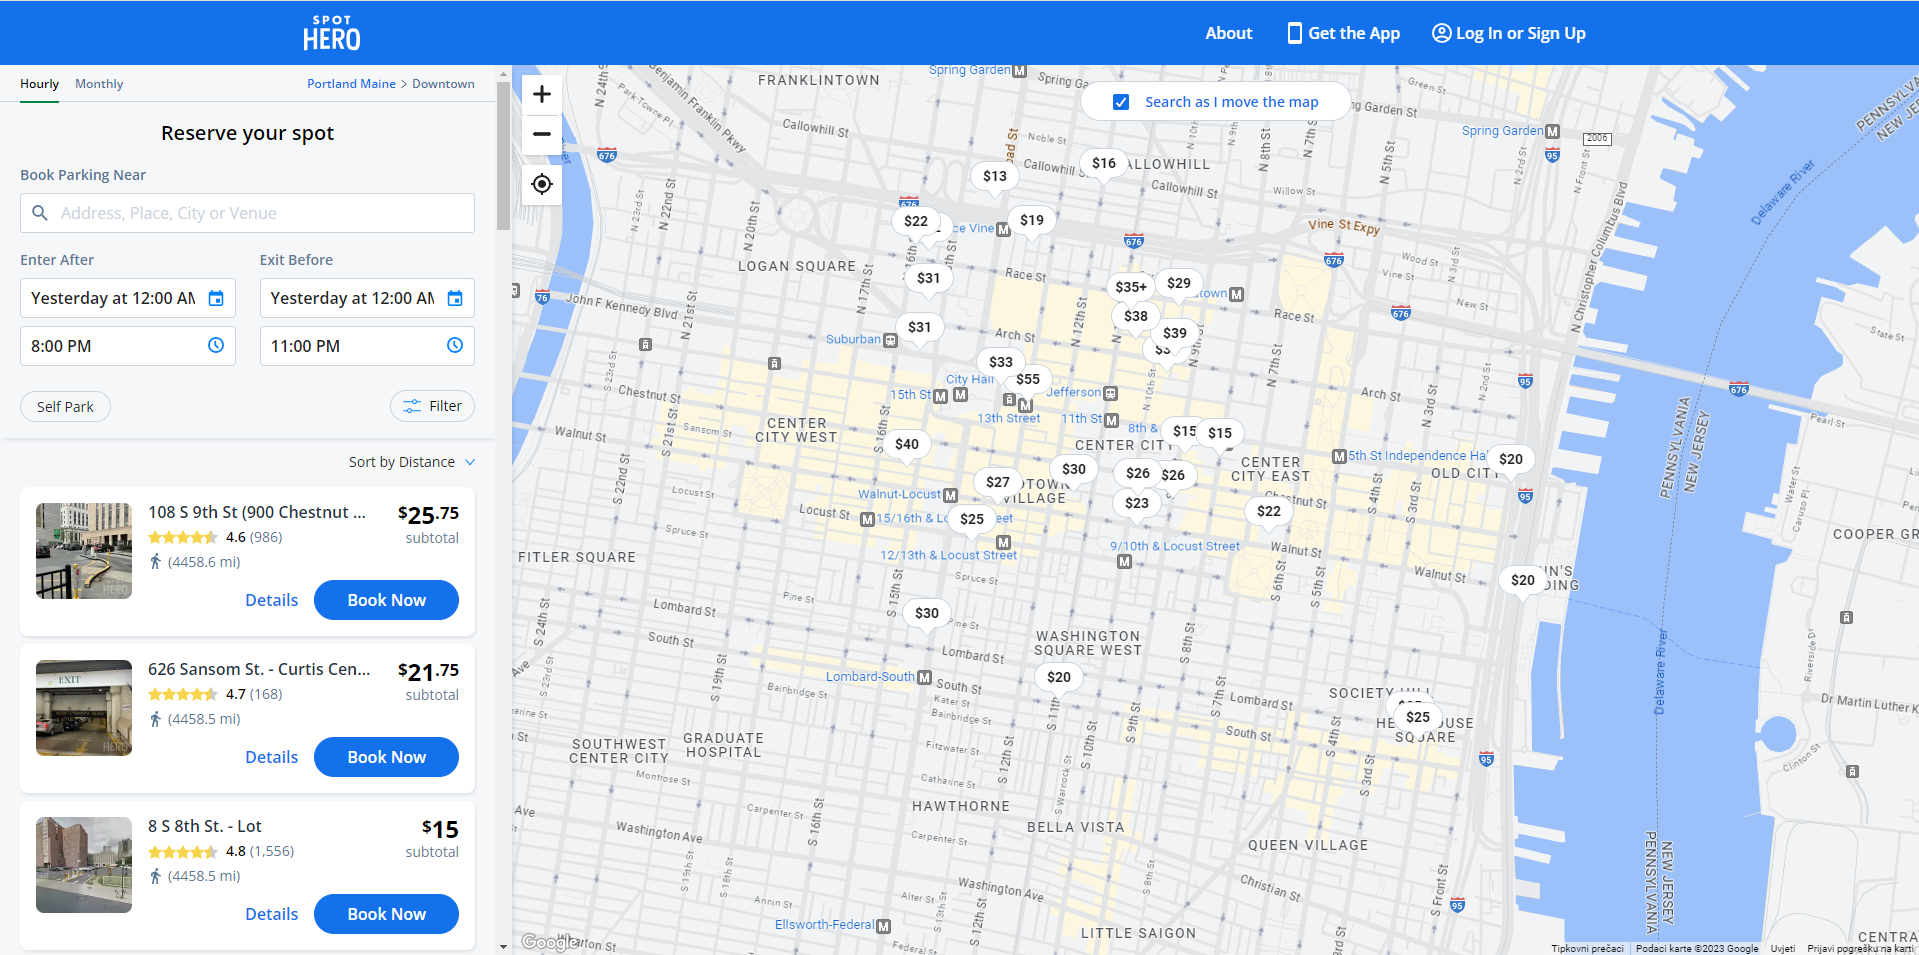
\includegraphics[width=\textwidth]{slike/spothero.PNG} 
			\caption{Prikaz aplikacije SpotHero}
			\label{fig:promjene3} 
		\end{figure}
		
		\begin{figure}[H]
			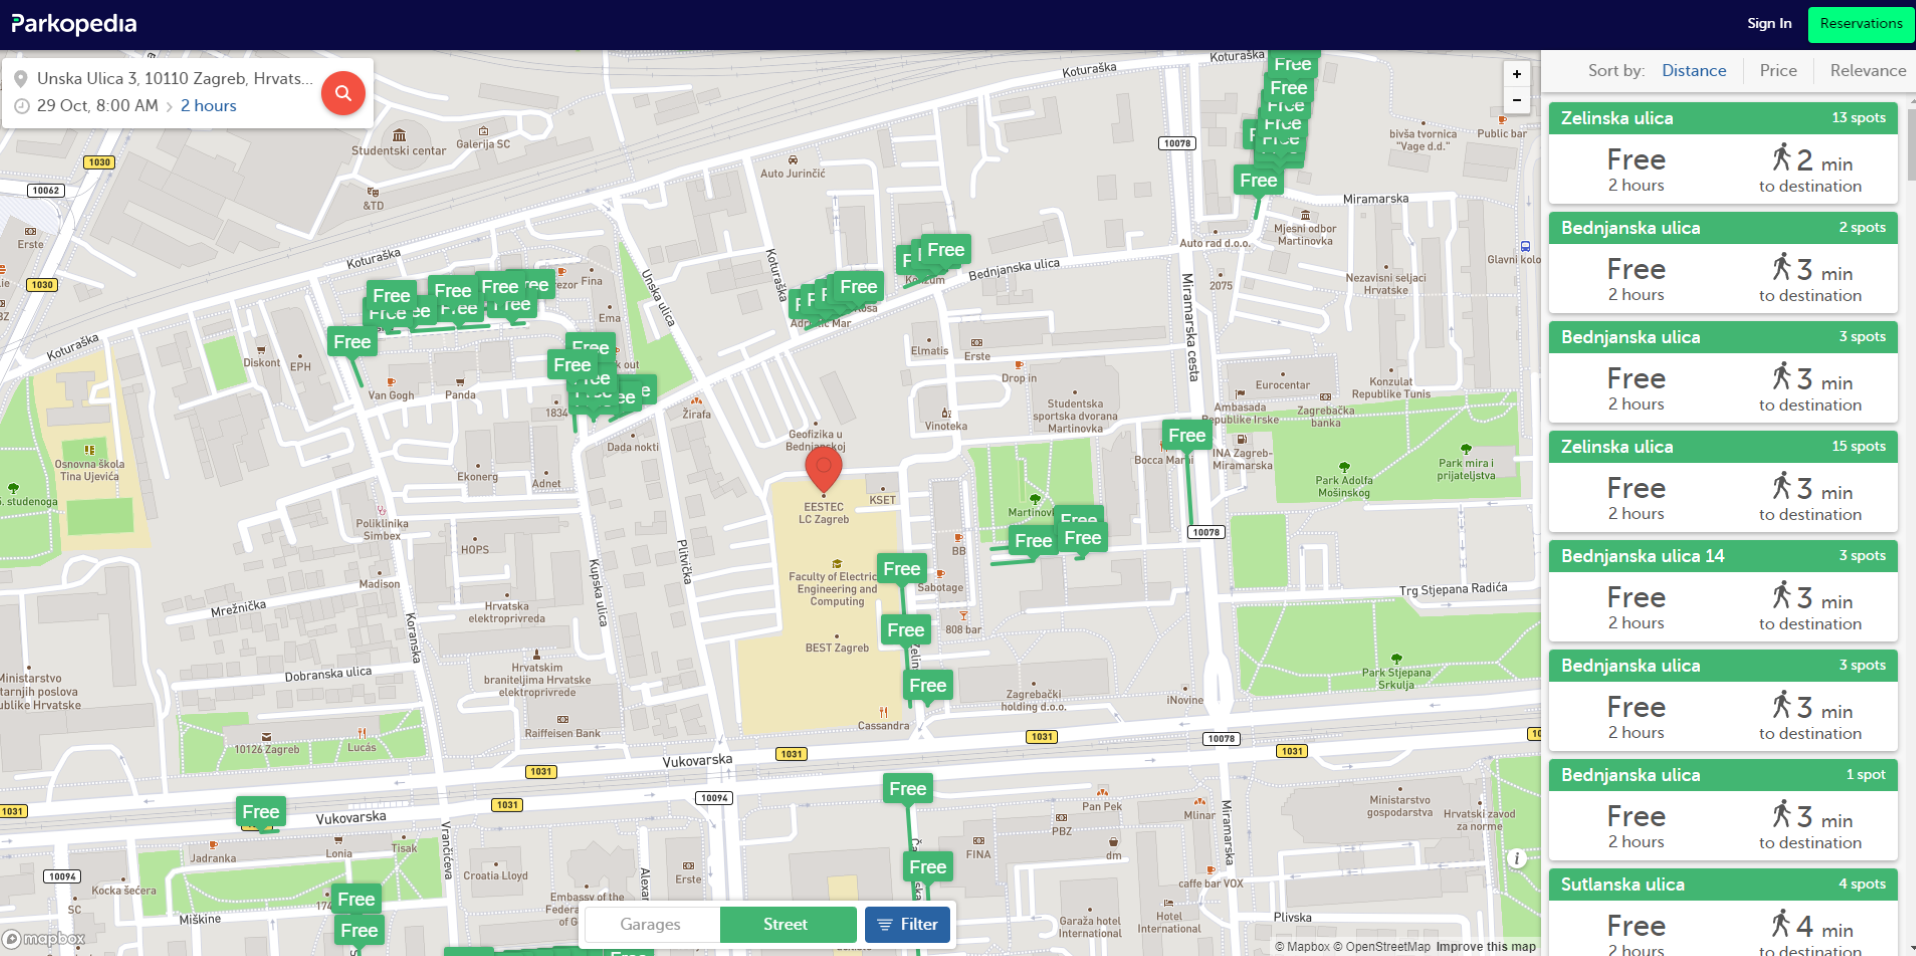
\includegraphics[width=\textwidth]{slike/parkopedia_street.PNG} 
			\caption{Prikaz aplikacije Parkopedia s označenim parkiralištima na ulici}
			\label{fig:promjene4} 
		\end{figure}
		
		\begin{figure}[H]
			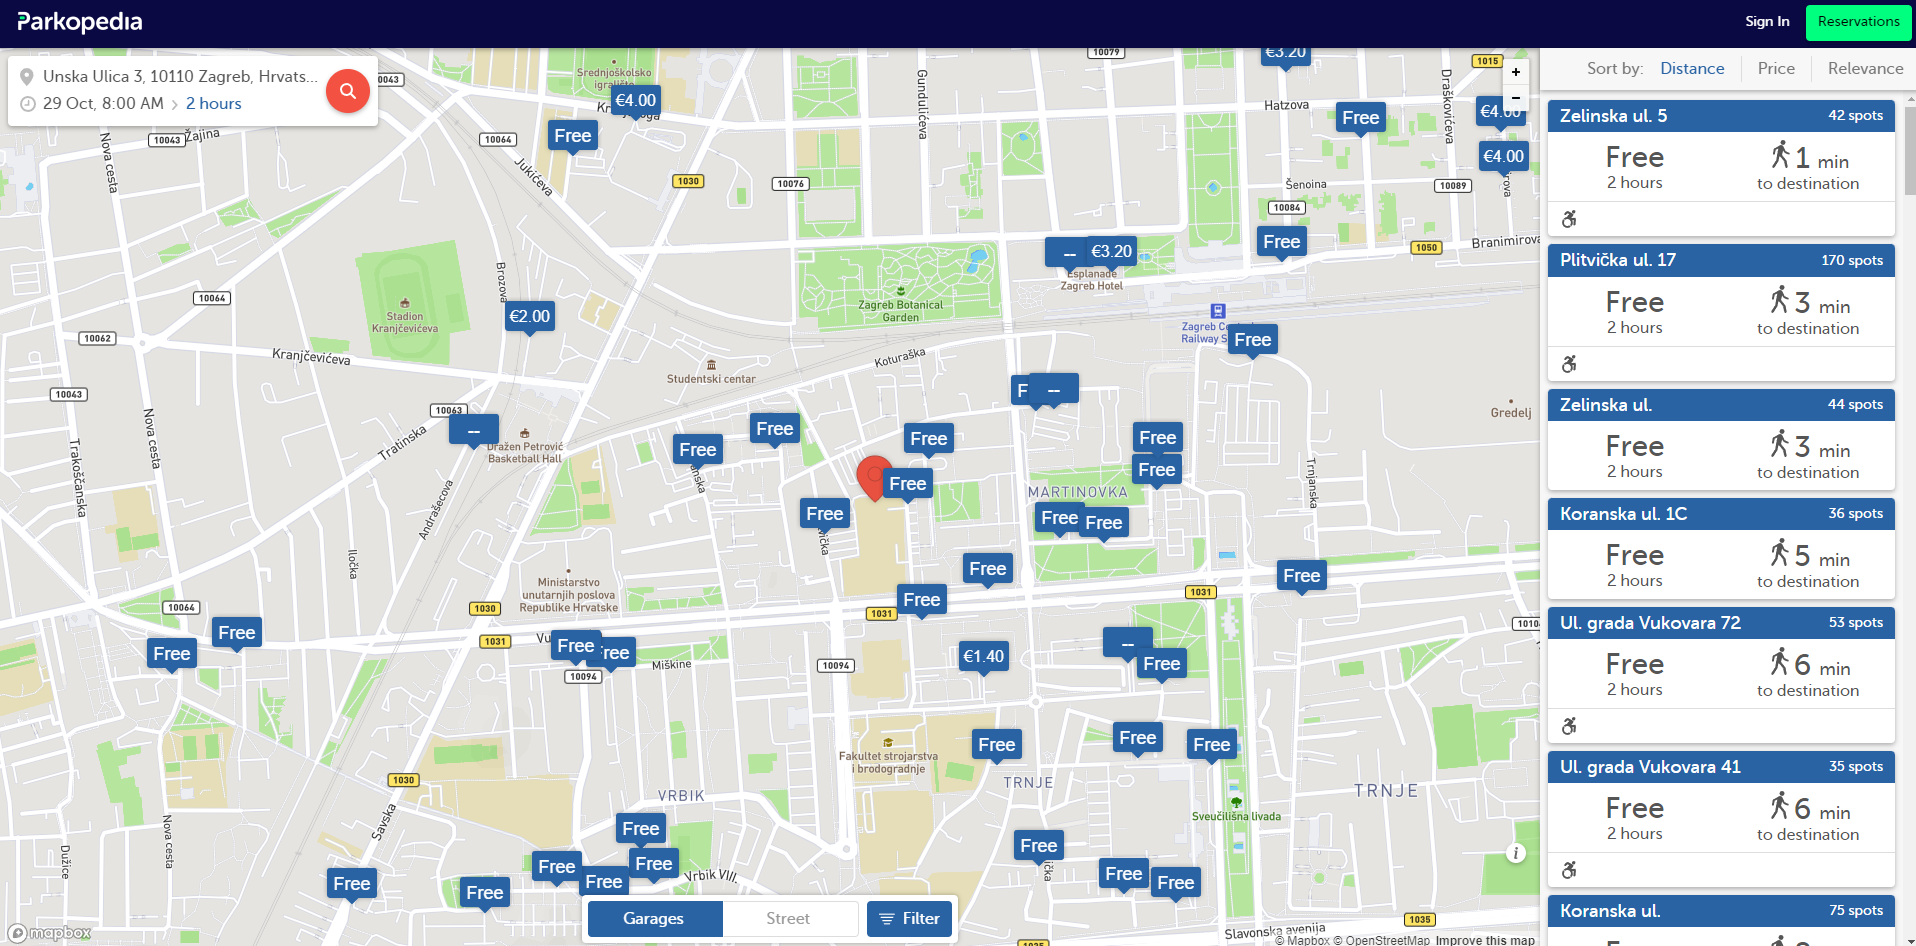
\includegraphics[width=\textwidth]{slike/parkopedia_garage.PNG}
			\caption{Prikaz aplikacije Parkopedia s označenim parkiralištima na garaži}
			\label{fig:promjene5} 
		\end{figure}
		
		Vjerujemo da našom aplikacijom možemo zainteresirati ljude koji su već upoznati s parking aplikacijama, ali smatraju da postoje područja u kojima trenutačno najpopularnije aplikacije nisu dovoljno prilagodljive korisničkim željama. Konačan plan i opseg ovog projekta je učiniti ovu aplikaciju dostupnu cijeloj Hrvatskoj. Ovisno o potrebi i potražnji korisnika, aplikaciju je moguće u budućnosti i nadograditi implementiranjem brojača slobodnih mjesta za bicikle.

		


		
		
	
	\chapter{Specifikacija programske potpore}
		
	\section{Funkcionalni zahtjevi}
			
			
			
			
			\noindent \textbf{Dionici:}
			
			\begin{packed_enum}
				
				\item Voditelj parkirališta
				\item Klijent			
				\item Administrator
                \item Razvojni tim
				
			\end{packed_enum}
			
			\noindent \textbf{Aktori i njihovi funkcionalni zahtjevi:}
			
			
			\begin{packed_enum}
				\item  \underbar{Neregistrirani korisnik (inicijator) može:}
				
				\begin{packed_enum}
					
					\item pregledati na karti pozicije svih parkirališta i dostupnim mjestima na parkiralištima
					\item poslati zahtjev za registraciju, a potrebni su: korisničko ime, lozinka, ime, prezime, slika osobne, IBAN račun i email adresa
					\begin{packed_enum}
						
						\item  moguće se registrirati kao klijent 
						\item  moguće se registrirati kao voditelj parkirališta
				
					\end{packed_enum}
					
					
				\end{packed_enum}
			
				\item  \underbar{Klijent (inicijator) može:}
				
				\begin{packed_enum}
					
					\item uz pregled parkirališta te dostupnih mjesta istih ima uvid u aktualnu zauzetost parkirnih mjesta
					\item unijeti odredište, tipa vozila i procijenjenu duljinu trajanja parkiranja čime generira rutu do najbližeg slobodnog parkirališta te rezervira parkirno mjesto ako postoji slobodno mjesto za rezervaciju
                        \item rezervirati parkiranje:
					\begin{packed_enum}
						
						\item  prema slobodnim terminima tražene lokacije
						\item  prema slobodnim lokacijama u traženom terminu
				
					\end{packed_enum}
                        \item nadopuniti novčanik sredstvima za plaćanje parkiranja
                        \item pregledavati i mijenjati osobne podatke
                        \item obrisati račun
					
				\end{packed_enum}
			\end{packed_enum}
   

                \begin{packed_enum}
				\item  \underbar{Voditelj parkirališta(inicijator) može:}
				
				\begin{packed_enum}
					
					\item unijeti informacije o svom parkiralištu (naziv, opis, fotografija, cjenik i sl.)
                        \begin{packed_enum}
						
						\item  u kartu ucrtati svako dostupno parkirališno mjesto za to parkiralište
				
					\end{packed_enum}
					\item definirati je li moguće rezervirati parkirališno mjesto
					\item definirati cijenu ovisno o trajanju rezervacije
					\item pristupiti statistici zauzetosti parkirališta i parkirališnih mjesta kroz vrijeme
                        \item obrisati parkirno mjesto
                        \item mijenjati informacije o svom parkiralištu
                        \item obrisati račun
					
				\end{packed_enum}
                \end{packed_enum}

                \begin{packed_enum}
				\item  \underbar{Administrator (inicijator) može:}
				
				\begin{packed_enum}
					
					
					\item potvrditi neregistriranog korisnika kao voditelja parkirališta
					\item pristupiti statistici zauzetosti parkirališta i parkirališnih mjesta kroz vrijeme
					\item dodati ili obrisati parkiralište i parkirna mjesta
                        \item pristupiti i izmijeniti podatke o parkiralištu
                        \item korisnike brisati i mijenjati im razinu pristupa aplikaciji
                        \item obrisati parkiralište
					
				\end{packed_enum}
                \end{packed_enum}

                \begin{packed_enum}
				\item  \underbar{Baza podataka (sudionik):}
				
				\begin{packed_enum}
					
					
					\item pohranjuje sve podatke o korisnicima i njihovim ovlastima
					\item pohranjuje sve podatke o parkiralištima i stanja zauzetosti parkirališnih mjesta
					
					
				\end{packed_enum}
                \end{packed_enum}
			
			\eject 
			
			
				
			\subsection{Obrasci uporabe}
				
				\textbf{\textit{dio 1. revizije}}
				
				\subsubsection{Opis obrazaca uporabe}
					\textit{Funkcionalne zahtjeve razraditi u obliku obrazaca uporabe. Svaki obrazac je potrebno razraditi prema donjem predlošku. Ako u nekom koraku može doći do odstupanja, potrebno je to odstupanje opisati i po mogućnosti ponuditi rješenje kojim bi se tijek obrasca vratio na osnovni tijek.}\\
					

					\noindent \underbar{\textbf{UC1 -Pregled parkirališta i parkirališnih mjesta na karti}}
					\begin{packed_item}
	
						\item \textbf{Glavni sudionik: }Klijent, Neregistrirani korisnik
						\item  \textbf{Cilj:} Pregledati dostupna parkirna mjesta
						\item  \textbf{Sudionici:} Baza podataka
						\item  \textbf{Preduvjet:} -
						\item  \textbf{Opis osnovnog tijeka:}
						
						\item[] \begin{packed_enum}
	
							\item Učitavanjem aplikacije prikazuje se karta s ucrtanim parkiralištima
							\item Korisnik odabire parkiralište
							\item Prikazuju se dostupna parkirališna mjesta za odabrano parkiralište te informacije o parkiralištu
							
						\end{packed_enum}

                            \item  \textbf{Opis mogućih odstupanja:}
						
						\item[] \begin{packed_item}
	
							\item[3.a] Glavni sudionik je registrirani Klijent
							\item[] \begin{packed_enum}
								
								\item Dodatno se prikazuje zauzetost parkirališnih mjesta u stvarnom vremenu
								
								
							\end{packed_enum}
	
							
						\end{packed_item}	
					\end{packed_item}

                        \noindent \underbar{\textbf{UC2 -Registracija}}
					\begin{packed_item}
	
						\item \textbf{Glavni sudionik: }Neregistrirani korisnik
						\item  \textbf{Cilj:} Stvoriti korisnički račun za pristup sustavu
						\item  \textbf{Sudionici:} Baza podataka
						\item  \textbf{Preduvjet:} -
						\item  \textbf{Opis osnovnog tijeka:}
						
						\item[] \begin{packed_enum}
	
							\item Korisnik odabire opciju za registraciju
							\item Korisnik unosi potrebne korisničke podatke
							\item Korisnik odabire vrstu registracije
							\item Korisnik registraciju potvrđuje preko maila
							
						\end{packed_enum}
						
						\item  \textbf{Opis mogućih odstupanja:}
						
						\item[] \begin{packed_item}

							\item[2.a] Odabir već zauzetog korisničkog imena i/ili e-maila, unos korisničkog podatka u nedozvoljenom formatu ili pružanje neispravnoga e-maila
							\item[] \begin{packed_enum}

									\item Sustav upozorava korisnika na probleme u registraciji i vraća ga na stranicu registracije
	
							\item[3.a] Odabrana je registracija računa Voditelja parkirališta
							\item[] \begin{packed_enum}
								
								\item Administrator mora dodatno potvrditi takvu registraciju
								
								
							\end{packed_enum}
	
							
						\end{packed_item}
					\end{packed_item}

                        \noindent \underbar{\textbf{UC3 -Prijava u sustav}}
					\begin{packed_item}
	
						\item \textbf{Glavni sudionik: }Klijent
						\item  \textbf{Cilj:} Dobiti pristup korisničkom sučelju
						\item  \textbf{Sudionici:} Baza podataka
						\item  \textbf{Preduvjet:} Registracija
						\item  \textbf{Opis osnovnog tijeka:}
						
						\item[] \begin{packed_enum}
	
							\item Unos korisničkog imena i lozinke
							\item Potvrda o ispravnosti unesenih podataka
							\item Pristup korisničkim funkcijama
							
						\end{packed_enum}

                            \item  \textbf{Opis mogućih odstupanja:}
						
						\item[] \begin{packed_item}
	
							\item[2.a] Neispravno korisničko ime/lozinka
							\item[] \begin{packed_enum}
								
								\item Sustav obavještava korisnika o neuspjelom upisu i vraća ga na stranicu za prijavu
								
								
							\end{packed_enum}
	
							
						\end{packed_item}	
					\end{packed_item}

                        \noindent \underbar{\textbf{UC4 -Pregled osobnih podataka}}
					\begin{packed_item}
	
						\item \textbf{Glavni sudionik: }Klijent
						\item  \textbf{Cilj:} Pregledati osobne podatke
						\item  \textbf{Sudionici:} Baza podataka
						\item  \textbf{Preduvjet:} Klijent je prijavljen
						\item  \textbf{Opis osnovnog tijeka:}
						
						\item[] \begin{packed_enum}
	
							\item Korisnik odabire opciju ”Osobni podatci”
							\item Otvara se stranica s osobnim podacima korisnika
							
							
						\end{packed_enum}

                    
					\end{packed_item}

                        \noindent \underbar{\textbf{UC5 -Promjena osobnih podataka}}
					\begin{packed_item}
	
						\item \textbf{Glavni sudionik: }Klijent
						\item  \textbf{Cilj:} Promijeniti osobne podatke
						\item  \textbf{Sudionici:} Baza podataka
						\item  \textbf{Preduvjet:} Klijent je prijavljen
						\item  \textbf{Opis osnovnog tijeka:}
						
						\item[] \begin{packed_enum}

							\item Korisnik odabire opciju ”Osobni podatci”
							\item Otvara se stranica s osobnim podacima korisnika
							\item Korisnik odabere opciju za promjenu podataka
							\item Korisnik mijenja svoje osobne podatke
							\item Korisnik sprema promjene
                                \item Baza podataka se ažurira
							
						\end{packed_enum}

                            \item  \textbf{Opis mogućih odstupanja:}
						
						\item[] \begin{packed_item}
	
							\item[2.a] Korisnik promijeni svoje osobne podatke, ali ne odabere opciju ”Spremi promjene”

							\item[] \begin{packed_enum}
								
								\item Sustav obavještava korisnika da nije spremio podatke prije izlaska iz prozora
								
								
							\end{packed_enum}
	
							
						\end{packed_item}	
					\end{packed_item}

                        \noindent \underbar{\textbf{UC6 -Brisanje korisničkog računa}}
					\begin{packed_item}
	
						\item \textbf{Glavni sudionik: }Klijent
						\item  \textbf{Cilj:} Obrisati korisnički račun
						\item  \textbf{Sudionici:} Baza podataka
						\item  \textbf{Preduvjet:} Klijent je prijavljen
						\item  \textbf{Opis osnovnog tijeka:}
						
						\item[] \begin{packed_enum}
	
							\item Korisnik odabire opciju ”Osobni podatci”
							\item Otvara se stranica s osobnim podacima korisnika
							\item Korisnik odabere opciju brisanja računa
                                \item Korisnički račun se izbriše iz baze podataka
                                \item Otvara se stranica za registraciju
							
						\end{packed_enum}

					\end{packed_item}
                            

					\noindent \underbar{\textbf{UC7 -Rezervacija parkirnog mjesta}}
					\begin{packed_item}
	
						\item \textbf{Glavni sudionik: }Klijent
						\item  \textbf{Cilj:} Rezervirati parkirališno mjesto
						\item  \textbf{Sudionici:} Baza podataka
						\item  \textbf{Preduvjet:} Klijent je prijavljen, Klijent (ili aplikacija) je odabrao mjesto, datum i vrijeme parkiranja
						\item  \textbf{Opis osnovnog tijeka:}
						
						\item[] \begin{packed_enum}
	
							\item Baza podataka zapiše podatke o rezervaciji
                            \item Parkiranje se naplati pri rezervaciji ili po dolasku na parkirališno mjesto
							
						\end{packed_enum}

						\item  \textbf{Opis mogućih odstupanja:}
						
						\item[] \begin{packed_item}
	
							\item[1.a] Klijent rezervaciju definira kao ponavljajuću
							\item[] \begin{packed_enum}
								
								\item Rezervacija se sprema u bazu podataka u posebnom obliku
								
								
							\end{packed_enum}
	
							
						\end{packed_item}	

					\end{packed_item}

                        \noindent \underbar{\textbf{UC8 -Odabir rezervacije parkirnog mjesta}}
					\begin{packed_item}
	
						\item \textbf{Glavni sudionik: }Klijent
						\item  \textbf{Cilj:} Rezervirati parkirališno mjesto
						\item  \textbf{Sudionici:} Baza podataka
						\item  \textbf{Preduvjet:} Klijent je prijavljen
						\item  \textbf{Opis osnovnog tijeka:}
						
						\item[] \begin{packed_enum}
	
							\item Klijent bira termin ili parkirališno mjesto te upisuje predviđeno trajanje rezervacije
							\item Ako je Klijent odabrao termin nude mu se odgovarajuća slobodna parkirališna mjesta, a ako je Klijent odabrao parkirališno mjesto nude mu se dostupni termini za dotično mjesto
							\item Klijent odabire mjesto, datum i trajanje rezervacije
                            \item Klijent odabire je li rezervacija ponavljajuća
							
						\end{packed_enum}

						\item  \textbf{Opis mogućih odstupanja:}
						
						\item[] \begin{packed_item}
	
							\item[1.a ILI 3.a] Klijent odabere današnji datum
							\item[] \begin{packed_enum}
								
								\item Sustav upozori korisnika da se ne može rezervirati mjesto na datum odabira
								
								
							\end{packed_enum}
	
							
						\end{packed_item}	

					\end{packed_item}

                        \noindent \underbar{\textbf{UC9 -Dohvat parkirališta}}
					\begin{packed_item}
	
						\item \textbf{Glavni sudionik: }Klijent
						\item  \textbf{Cilj:} Pronaći put do najbližeg parkirališta i rezervirati ako je moguće
						\item  \textbf{Sudionici:} Baza podataka
						\item  \textbf{Preduvjet:} Klijent je prijavljen
						\item  \textbf{Opis osnovnog tijeka:}
						
						\item[] \begin{packed_enum}
	
							\item Klijent odabire odredište na karti, tip vozila i procjenu trajanja parkiranja
							\item Aplikacija iscrta rutu na mapi do najbližeg slobodnog parkirališnog mjesta
							\item Mjesto se rezervira ako je slobodno za rezervaciju
							
						\end{packed_enum}
					\end{packed_item}

					\noindent \underbar{\textbf{UC10 -Pregled rezervacija}}
					\begin{packed_item}
	
						\item \textbf{Glavni sudionik: }Klijent
						\item  \textbf{Cilj:} Pregled aktivnih rezervacija
						\item  \textbf{Sudionici:} Baza podataka
						\item  \textbf{Preduvjet:} Klijent je prijavljen i napravio je barem jednu rezervaciju
						\item  \textbf{Opis osnovnog tijeka:}
						
						\item[] \begin{packed_enum}
	
							\item Klijent odabire opciju ”Moje rezervacije”
							\item Prikaže se lista rezervacija korisnika
							
						\end{packed_enum}
					\end{packed_item}

                        \noindent \underbar{\textbf{UC11 -Uređivanje rezervacije}}
					\begin{packed_item}
	
						\item \textbf{Glavni sudionik: }Klijent
						\item  \textbf{Cilj:} Uređivanje aktivne rezervacija
						\item  \textbf{Sudionici:} Baza podataka
						\item  \textbf{Preduvjet:} Klijent je prijavljen i napravio je barem jednu rezervaciju
						\item  \textbf{Opis osnovnog tijeka:}
						
						\item[] \begin{packed_enum}
	
							\item Klijent odabire opciju ”Moje rezervacije”
							\item Prikaže se lista rezervacija korisnika
							\item Klijent odabire rezervaciju koju želi urediti
                                \item Prikaže se lista dostupnih parkirnih mjesta i slobodnih termina za iste
                                \item Korisnik čini promjene te ih sprema
							
						\end{packed_enum}
					\end{packed_item}

                        \noindent \underbar{\textbf{UC12 -Brisanje rezervacije}}
					\begin{packed_item}
	
						\item \textbf{Glavni sudionik: }Klijent
						\item  \textbf{Cilj:} Otkazati zakazanu rezervaciju
						\item  \textbf{Sudionici:} Baza podataka
						\item  \textbf{Preduvjet:} Klijent je prijavljen i postoji barem jedna aktualna rezervacija
						\item  \textbf{Opis osnovnog tijeka:}
						
						\item[] \begin{packed_enum}
	
							\item Klijent odabire opciju ”Moje rezervacije”
							\item Prikaže se lista rezervacija korisnika
							\item Klijent bira opciju za brisanje rezervacije
                                \item Rezervacija se uklanja iz Baze podataka
							
						\end{packed_enum}
					\end{packed_item}

						\noindent \underbar{\textbf{UC13 -Plačanje}}
					\begin{packed_item}
	
						\item \textbf{Glavni sudionik: }Klijent
						\item  \textbf{Cilj:} Platiti parkiranje
						\item  \textbf{Sudionici:} Baza podataka, Voditelj parkirališta
						\item  \textbf{Preduvjet:} Klijent je prijavljen, parkiralište se plača aplikacijom
						\item  \textbf{Opis osnovnog tijeka:}
						
						\item[] \begin{packed_enum}
	
							\item Uzme se određena količina iz računa Klijenta
							\item Stavlja se na račun Voditelja parkirališta koje se rezervira
							\item Rezervacija se označi plačenom 
							
							
						\end{packed_enum}

						\item  \textbf{Opis mogućih odstupanja:}
						
						\item[] \begin{packed_item}
	
							\item[1.a] Klijent nema dovoljno novca na računu
							\item[] \begin{packed_enum}
								
								\item Sustav upozori korisnika da nema dovoljno novca
								\item Sustav prekine sa tijekom izvođenja
								
								
							\end{packed_enum}
	
							
						\end{packed_item}	

					\end{packed_item}

						\noindent \underbar{\textbf{UC14 -Uplata}}
					\begin{packed_item}
	
						\item \textbf{Glavni sudionik: }Klijent
						\item  \textbf{Cilj:} Uplatiti novac na račun
						\item  \textbf{Sudionici:} Baza podataka
						\item  \textbf{Preduvjet:} Klijent je prijavljen
						\item  \textbf{Opis osnovnog tijeka:}
						
						\item[] \begin{packed_enum}
	
							\item Klijent odabere opciju uplate novca
							\item Klijent upiše podatke računa/kartica s koje se uzima novac i kolko novca želi prenijeti
							\item Potvrđuje se transakcija
							\item Dodaju se novi novci na račun
							
							
						\end{packed_enum}

						\item  \textbf{Opis mogućih odstupanja:}
						
						\item[] \begin{packed_item}
	
							\item[2.a] Krivo upisane informacije računa/kartice
							\item[] \begin{packed_enum}
								
								\item Sustav upozori korisnika da je krivo upisao podatke
								\item Sustav vrati korisnika na stranicu upisa podataka
								
								
							\end{packed_enum}

							\item[3.a] Nedovoljno novca na računu
							\item[] \begin {packed_enum}

								\item Sustav ipozori korisnika da nema dovoljno novca na računu
								\item Sustav vrati korisnika na stranicu upisa podataka

						\end{packed_enum}
	
							
						\end{packed_item}	

					\end{packed_item}

                        \noindent \underbar{\textbf{UC15 -Pregled aktivnih rezervacija parkirališta}}
					\begin{packed_item}
	
						\item \textbf{Glavni sudionik: }Voditelj parkirališta
						\item  \textbf{Cilj:} Pregledati sve aktualne rezervacije
						\item  \textbf{Sudionici:} Baza podataka
						\item  \textbf{Preduvjet:} Rezervacije su zaprimljene i plaćene
						\item  \textbf{Opis osnovnog tijeka:}
						
						\item[] \begin{packed_enum}
	
							\item Voditelj odabere opciju pregleda aktivnih rezervaciju
							\item Prikaže se lista aktivnih rezervacija
						
						\end{packed_enum}
					\end{packed_item}

                        \noindent \underbar{\textbf{UC16 -Ucrtavanje novog parkirnog mjesta}}
					\begin{packed_item}
	
						\item \textbf{Glavni sudionik: }Voditelj parkirališta
						\item  \textbf{Cilj:} Ucrtati novo parkirno mjesto u sklopu postojećeg parkirališta
						\item  \textbf{Sudionici:} Baza podataka
						\item  \textbf{Preduvjet:} Voditelj je prijavljen
						\item  \textbf{Opis osnovnog tijeka:}
						
						\item[] \begin{packed_enum}
	
							\item Voditelj odabire opciju prikaza tlocrta parkirališta
							\item Prikazuje mu se tlocrt parkirališta
							\item Voditelj odabire opciju za ucrtavanje novog parkirnog mjesta
                                \item Voditelj ucrtava na tlocrt novo parkirno mjesto
                                \item promjene se upisuju u Bazu podataka
							
						\end{packed_enum}
					\end{packed_item}

                        \noindent \underbar{\textbf{UC17 -Uređivanje podacima o parkiralištu}}
					\begin{packed_item}
	
						\item \textbf{Glavni sudionik: }Voditelj parkirališta
						\item  \textbf{Cilj:} Izmijeniti informacije o parkiralištu
						\item  \textbf{Sudionici:} Baza podataka
						\item  \textbf{Preduvjet:} Voditelj parkirališta je prijavljen
						\item  \textbf{Opis osnovnog tijeka:}
						
						\item[] \begin{packed_enum}
	
							\item Voditelj parkirališta bira prikaz opciju prikaza informacija o parkiralištu
							\item Prikazuju mu se ranije unesene informacije
							\item Voditelj bira opciju izmjene dotičnih podataka 
                                \item Izmijenjeni podatci se spremaju u Bazu podataka
							
						\end{packed_enum}
					\end{packed_item}


                        \noindent \underbar{\textbf{UC18 -Uklanjanje parkirnog mjesta}}
					\begin{packed_item}
	
						\item \textbf{Glavni sudionik: }Voditelj parkirališta
						\item  \textbf{Cilj:} Ukloniti željena parkirna mjesta
						\item  \textbf{Sudionici:} Baza podataka
						\item  \textbf{Preduvjet:} Voditelj parkirališta je prijavljen, postoje ucrtana parkirna mjesta
						\item  \textbf{Opis osnovnog tijeka:}
						
						\item[] \begin{packed_enum}
	
							\item Voditelj bira opciju prikaza tlocrta parkirališta
							\item Voditelj potom bira opciju uklanjanja parkirnog mjesta
							\item Odabrana uklonjena parkirna mjesta se uklanjaju iz Baze podataka
							
						\end{packed_enum}

        
					\end{packed_item}

                        \noindent \underbar{\textbf{UC19 -Potvrđivanje voditelja parkirališta}}
					\begin{packed_item}
	
						\item \textbf{Glavni sudionik: }Administrator
						\item  \textbf{Cilj:} Potvrditi registraciju računa Voditelja parkirališta
						\item  \textbf{Sudionici:} Baza podataka
						\item  \textbf{Preduvjet:} Prijavljen je administrator i postoji nepotvrđena registracija za račun Voditelja parkirališta
						\item  \textbf{Opis osnovnog tijeka:}
						
						\item[] \begin{packed_enum}
	
							\item Administrator otvara listu registraciju na čekanju
							\item Administrator potvrđuje određene registracije
							\item U bazu podataka se spremaju promijene
							
						\end{packed_enum}

        	
					\end{packed_item}

                        \noindent \underbar{\textbf{UC20 -Pregled Korisnika}}
					\begin{packed_item}
	
						\item \textbf{Glavni sudionik: }Administrator
						\item  \textbf{Cilj:} Pregledati registrirane korisnike
						\item  \textbf{Sudionici:} Baza podataka
						\item  \textbf{Preduvjet:} Prijavljeni korisnik ima administratorska prava
						\item  \textbf{Opis osnovnog tijeka:}
						
						\item[] \begin{packed_enum}
	
							\item Administrator odabire opciju pregledavanja korisnika
							\item Prikaže se lista svih ispravno registriranih korisnika s osobnim podacima
			
						\end{packed_enum}

                    
					\end{packed_item}

                        \noindent \underbar{\textbf{UC21 -Brisanje korisnika}}
					\begin{packed_item}
	
						\item \textbf{Glavni sudionik: }Administrator
						\item  \textbf{Cilj:} Ukloniti korisnika iz Baze podataka
						\item  \textbf{Sudionici:} Baza podataka
						\item  \textbf{Preduvjet:} Prijavljeni korisnik ima administratorska prava
						\item  \textbf{Opis osnovnog tijeka:}
						
						\item[] \begin{packed_enum}
	
							\item Administrator odabire opciju uklanjanja korisnika
							\item Administrator pronalazi željenog korisnika
							\item Administrator uklanja željenog korisnika i njegove podatke iz baze podataka
							
						\end{packed_enum}

					\end{packed_item}

                        \noindent \underbar{\textbf{UC22 -Promjena prava pristupa}}
					\begin{packed_item}
	
						\item \textbf{Glavni sudionik: }Administrator
						\item  \textbf{Cilj:} Promijeniti prava korisnika
						\item  \textbf{Sudionici:} Baza podataka
						\item  \textbf{Preduvjet:} 						
						\item  \textbf{Preduvjet:} Prijavljeni korisnik ima administratorska prava
						\item  \textbf{Opis osnovnog tijeka:}
						
						\item[] \begin{packed_enum}
	
							\item Administrator pronalazi željenog korisnika
							\item Administrator mijenja razinu pristupa željenom korisniku
							
							
						\end{packed_enum}

					\end{packed_item}

                        \noindent \underbar{\textbf{UC23 -Pregled statistike}}
					\begin{packed_item}
	
						\item \textbf{Glavni sudionik: }Voditelj parkirališta
						\item  \textbf{Cilj:} Pregledati statistiku popunjenosti parkirališnih mjesta
						\item  \textbf{Sudionici:} Baza podataka
						\item  \textbf{Preduvjet:} Korisnik je prijavljen kao Voditelj parkirališta
						\item  \textbf{Opis osnovnog tijeka:}
						
						\item[] \begin{packed_enum}
	
							\item Izabere se opcija prikaza statistike za parkiralište
							\item Prikazuje se statistika zauzetosti mjesta dotičnog parkirališta
							
							
						\end{packed_enum}

					\end{packed_item}

				
					
				\subsubsection{Dijagrami obrazaca uporabe}
					
					\begin{figure}[H]
						\centering
						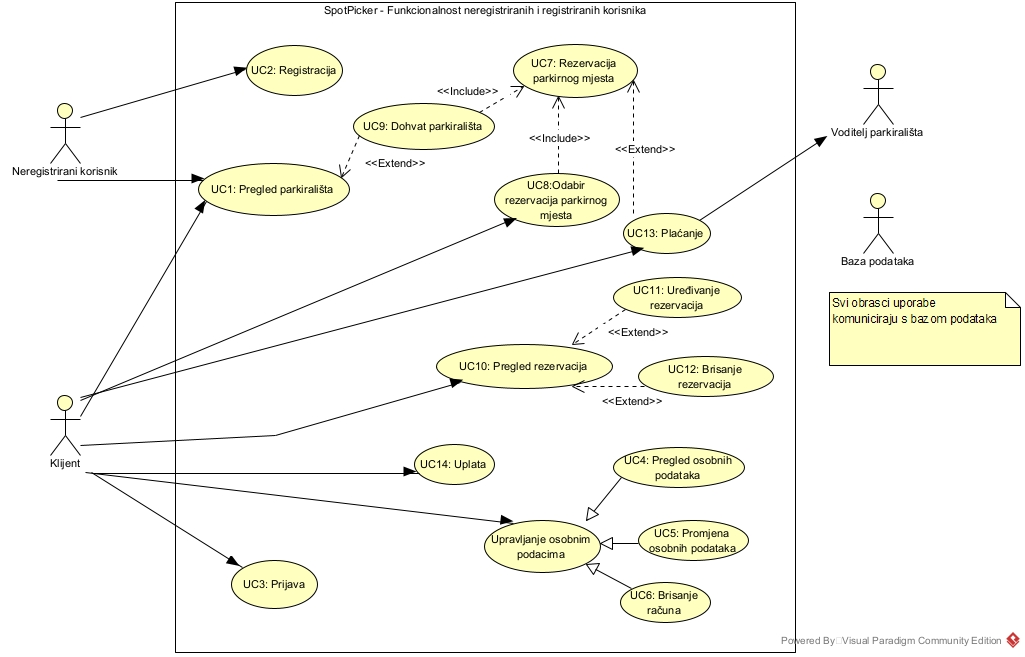
\includegraphics[width=\textwidth]{slike/UCD1.PNG} 
						\caption{Dijagram obrasca uporabe, funkcionalnost neregistriranih i registriranih korisnika}
						\label{fig:promjene6} 
					\end{figure}
					
					\begin{figure}[H]
						\centering
						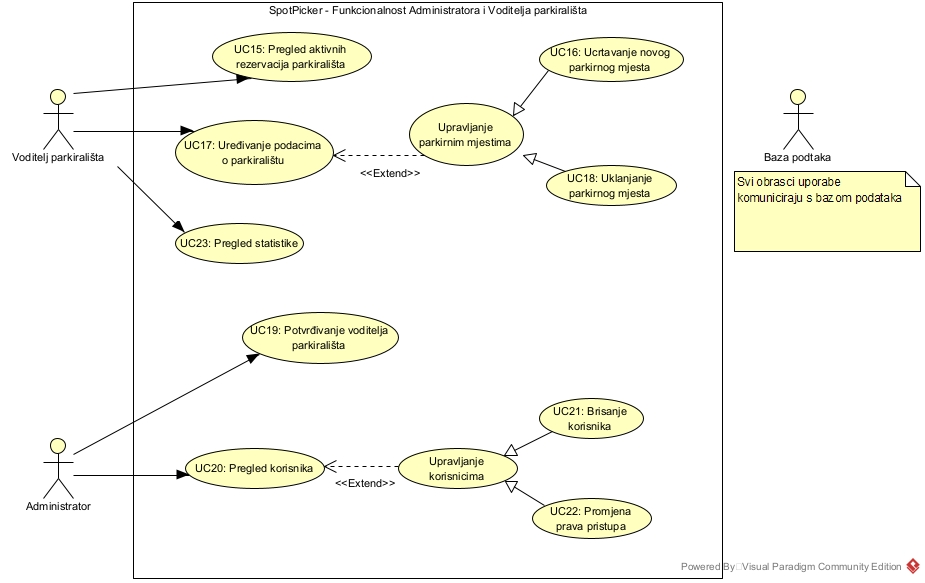
\includegraphics[width=\textwidth]{slike/UCD2.PNG} 
						\caption{Dijagram obrasca uporabe, funkcionalnost administratora i voditelja parkirališta}
						\label{fig:promjene7} 
					\end{figure}
				\eject		
				
			\subsection{Sekvencijski dijagrami}
				
				\begin{figure}[H]
					\centering
					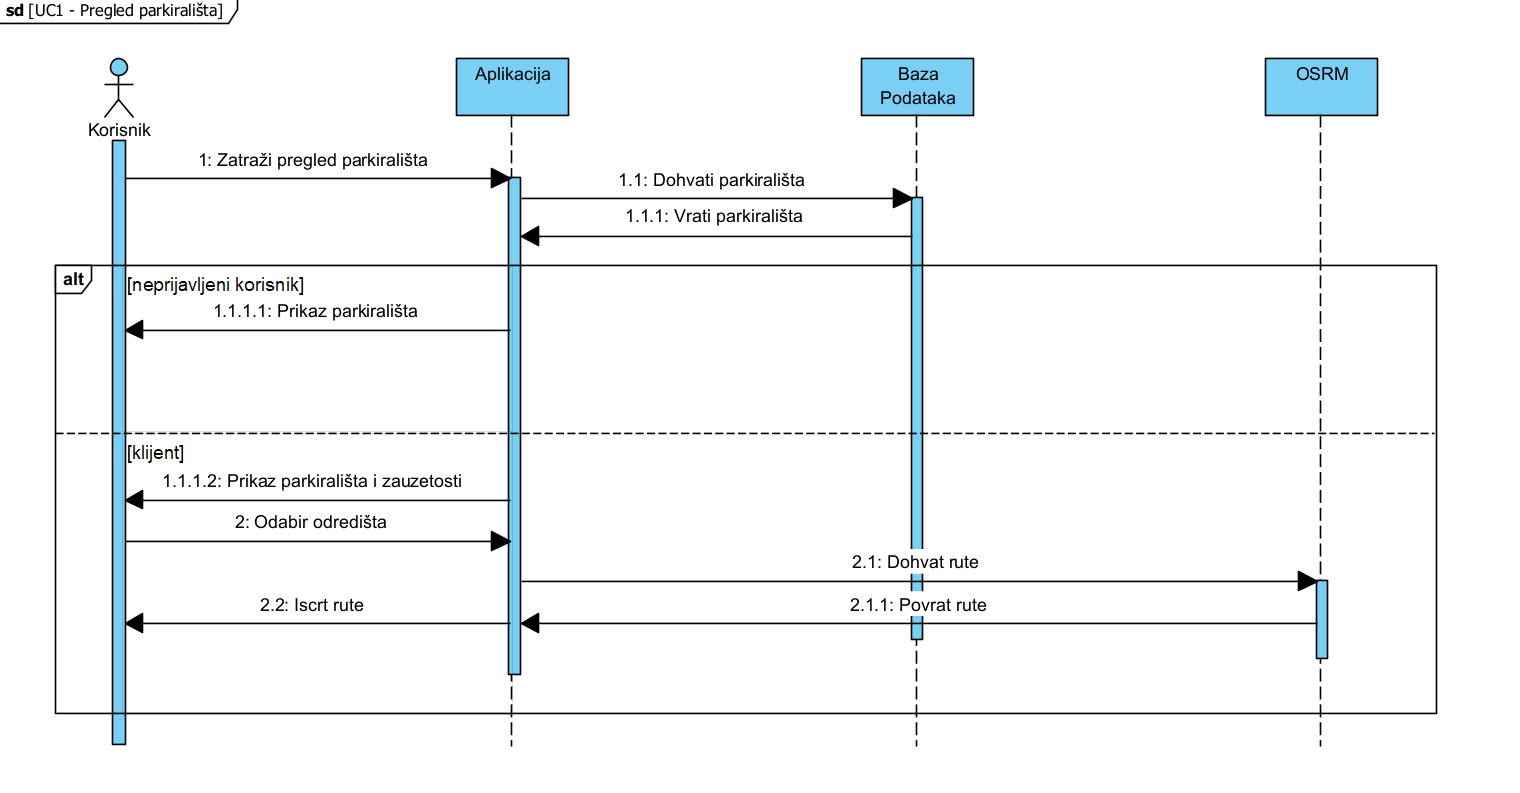
\includegraphics[width=\textwidth]{slike/SD_UC1.JPG} 
					\caption{Sekvencijski dijagram za UC1}
					\label{fig:promjene8} 
				\end{figure}
				
				\begin{figure}[H]
					\centering
					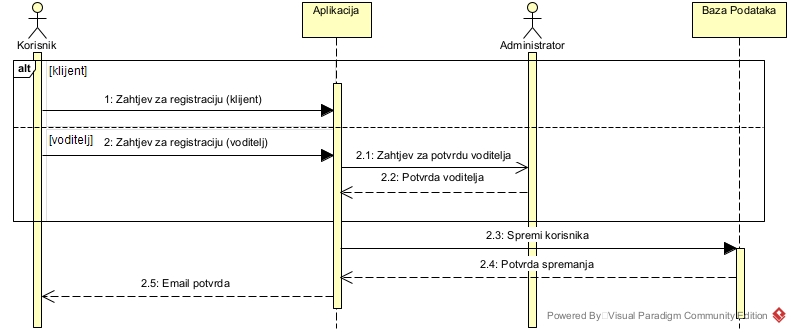
\includegraphics[width=\textwidth]{slike/SD_UC2.JPG} 
					\caption{Sekvencijski dijagram za UC2}
					\label{fig:promjene9} 
				\end{figure}
				
				\begin{figure}[H]
					\centering
					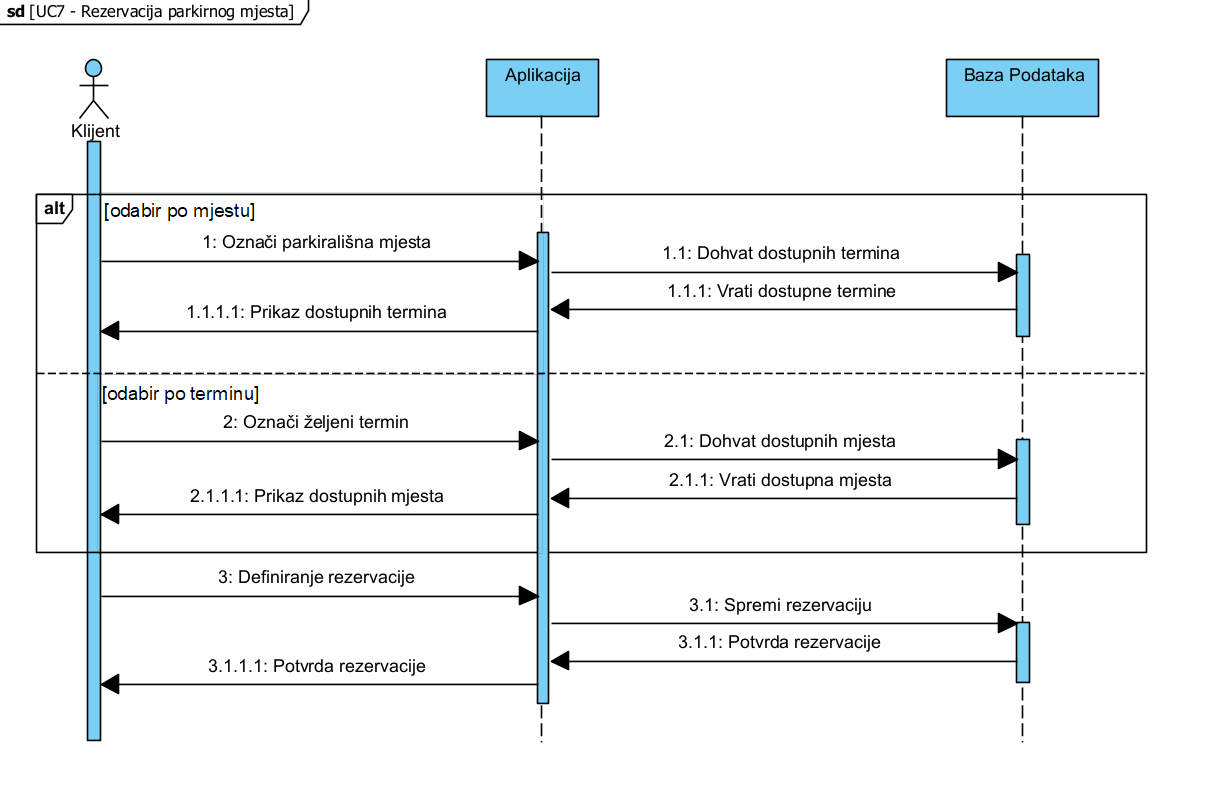
\includegraphics[width=\textwidth]{slike/SD_UC7.JPG} 
					\caption{Sekvencijski dijagram za UC7}
					\label{fig:promjene10} 
				\end{figure}
				
				\begin{figure}[H]
					\centering
					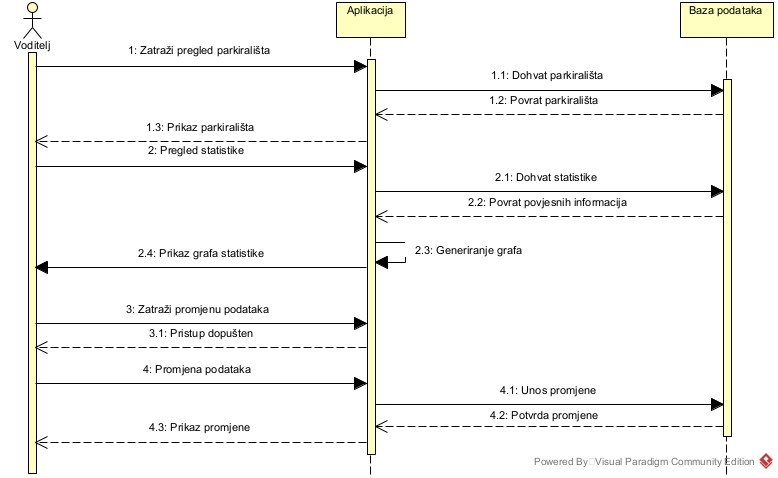
\includegraphics[width=\textwidth]{slike/SD_UC17.JPG} 
					\caption{Sekvencijski dijagram za UC17}
					\label{fig:promjene11} 
				\end{figure}
				\eject
	
		\section{Ostali zahtjevi}
		
			\textbf{\textit{dio 1. revizije}}\\
		 
			 \textit{Nefunkcionalni zahtjevi i zahtjevi domene primjene dopunjuju funkcionalne zahtjeve. Oni opisuju \textbf{kako se sustav treba ponašati} i koja \textbf{ograničenja} treba poštivati (performanse, korisničko iskustvo, pouzdanost, standardi kvalitete, sigurnost...). Primjeri takvih zahtjeva u Vašem projektu mogu biti: podržani jezici korisničkog sučelja, vrijeme odziva, najveći mogući podržani broj korisnika, podržane web/mobilne platforme, razina zaštite (protokoli komunikacije, kriptiranje...)... Svaki takav zahtjev potrebno je navesti u jednoj ili dvije rečenice.}
			 \begin{packed_enum}

				\item Koristiti OSRM za dohvat rute na mapi
				\item Koristiti Overpass API za dohvat početne informacije o parkirališnim mjestima
				\item Sustav mora biti implementiran kao web aplikacija koristeći isključivo objektno-orijentirane jezike
				\item Statistika parkirališta se prikazuje u obliku grafa
				
			 \end{packed_enum}
			 
			 
	\chapter{Arhitektura i dizajn sustava}
		
		\textbf{\textit{dio 1. revizije}}\\

		\textit{ Potrebno je opisati stil arhitekture te identificirati: podsustave, preslikavanje na radnu platformu, spremišta podataka, mrežne protokole, globalni upravljački tok i sklopovsko-programske zahtjeve. Po točkama razraditi i popratiti odgovarajućim skicama:}
	\begin{itemize}
		\item 	\textit{izbor arhitekture temeljem principa oblikovanja pokazanih na predavanjima (objasniti zašto ste baš odabrali takvu arhitekturu)}
		\item 	\textit{organizaciju sustava s najviše razine apstrakcije (npr. klijent-poslužitelj, baza podataka, datotečni sustav, grafičko sučelje)}
		\item 	\textit{organizaciju aplikacije (npr. slojevi frontend i backend, MVC arhitektura) }		
	\end{itemize}

	
		

		

				
		\section{Baza podataka}
			
			
		
		
		\subsection{Vrsta i implementacija}
		Za modeliranje sustava je korištena relacijska baza podataka, a nju smo implementirati pomoću open-source sustava za upravljanje bazama podataka PostgreSQL. Za izradu dijagrama ER i generiranje relacijske sheme je korišten besplatan online alat ERDplus (https://erdplus.com/) koji je korišten i u sklopu predmeta Baze podataka. 
		
		
		
		\subsection{Glavne komponente baze podataka}
		Baza podataka sastoji se od sljedećih entiteta:
		
		\begin{itemize}
			\item \textbf{Korisnik}\textit{Korisnicko\_ime}, \textit{Lozinka}, \textit{Ime}, \textit{Prezime}, \textit{Slika\_osobne}, \textit{IBAN}, \textit{email}, \textit{Uloga}, \textit{stanjeNaRacunu})
			
			
			\item \textbf{ParkiralisteAutomobili} (\textit{fotografija}, \textit{Naziv}, \textit{Opis}, \textit{CijenaPoSatu}, \textit{ParkiralisteId}) 
			
			\item \textbf{Parking\_mjesto} (\textit{identifikacija}, \textit{Oznaka}, \textit{Slobodno}, \textit{Dostupno}, \textit{ParkiralisteId})
			
			\item \textbf{Voditelj} (\textit{jePrihvacen}, \textit{korisnickoIme}, \textit{ParkiralisteId})
			
			\item \textbf{Rezervacija} (\textit{RezervacijaID}, \textit{cijena}, \textit{pocetakRezervacije}, \textit{krajRezervacije}, \textit{RRule}, \textit{KorisnickoIme}, \textit{Identifikacija})
			
			\item \textbf{BicikliMjesto} (\textit{identifikacija}, \textit{BrojMjesta}, \textit{duljina}, \textit{sirina})
		\end{itemize}
		
		
		
			\subsection{Opis tablica}
			

				
			
				
			\textbf{Korisnik:} sadržava sve bitne informacije o registriranim korisnicima u sustavu. Sadrži atribute: ID korisnika, korisničko ime, lozinka, ime, prezime, slika osobne iskaznice, IBAN, email, uloga (enum za 'klijent', 'voditelj', 'administrator') i stanje na računu. Ovaj entitet je preko korisnickogImena u vezi One-to-Many s entitetom Rezervacija i u One-to-One vezi s entitetom Voditelj.
				\begin{longtblr}[
					label=none,
					entry=none,
					]{
						width = \textwidth,
						colspec={|X[9,l]|X[5,l]|X[20, l]|},
						rowhead = 1,
					}
					\hline \SetCell[c=3]{c}{\textbf{Korisnik}} \\ \hline[3pt]	
					\SetCell{LightGreen} KorisničkoIme & VARCHAR & Jedinstveno korisničko ime \\ \hline
					email & VARCHAR & Email korisnika\\ \hline
					lozinka & VARCHAR & Hash lozinke dobiven s Bcrypt encoderom\\ \hline
					Ime & VARCHAR & Ime korisnika\\ \hline
					Prezime & VARCHAR & Prezime korisnika\\ \hline
					IBAN & VARCHAR &  IBAN korisnika\\ \hline
					slikaOsobne & BYTEA & Byte array slike osobne iskaznice\\ \hline
					Uloga & INT & Enum koji označava ulogu korisnika ('klijent', 'voditelj', 'administrator')\\ \hline
					stanjeNaRacunu & NUMERIC & Decimalni broj koji označava koliko novaca se nalazi u novčaniku \\ \hline
				
				\end{longtblr}
				
				
				
				\noindent\textbf{ParkiralisteAutomobili:} sadrži ključne informacije vezane za parkirališta automobila. Sadrži atribute koje postavlja voditelj parkirališta: fotografija, naziv, opis i cijena po satu. Uz to sadrži i ID parkirališta. Ovaj entitet je u vezi One-to-One s entitetom voditelj putem ID-a parkirališta i One-to-Many vezi s ParkingMjesto preko ID-a parkirališta.
				\begin{longtblr}[
					label=none,
					entry=none
					]{
						width = \textwidth,
						colspec={|X[6,l]|X[6, l]|X[20, l]|}, 
						rowhead = 1,
					}
					\hline \SetCell[c=3]{c}{\textbf{ParkiralisteAutomobili}} \\ \hline[3pt]
					\SetCell{LightGreen}ParkiralisteId & INT & Jedinstveni identifikator parkirališta\\ \hline
					fotografija & BYTEA & Slika parkirališta koju voditelj može priložiti\\ \hline
					Naziv & VARCHAR & Naziv parkirališta\\ \hline
					Opis & VARCHAR & Opis parkirališta\\ \hline
					CijenaPoSatu & NUMERIC & Cijena po satu koju definira voditelj parkirališta\\ \hline
				
				\end{longtblr}
				
				\noindent\textbf{Parking\_mjesto:} predstavlja informacije o pojedinačnim parkirnim mjestima unutar parkirališta za automobile. U ovu tablicu ćemo unijeti početne informacije o mjestima za automobile koje smo dobili od overpass API-ja.  Sadrži atribute kao što su identifikacija i koordinate (duljina, širina) koje ćemo dobiti pozivom overpassAPI-a. (@id i "coordinates" iz GeoJSON-a dobivenog pozivom overpassAPI-a), oznaka parkirnog mjesta, informacija o dostupnosti koju postavlja voditelj i slobodnom statusu parkirnog mjesta te ID parkirališta kojem pripada. U U vezi je Many-to-One s entitetom "ParkirališteAutomobili" putem ID-a parkirališta i One-to-many s entitetom Rezervacija putem identifikacije parking mjesta.
				\begin{longtblr}[
					label=none,
					entry=none
					]{
						width = \textwidth,
						colspec={|X[6,l]|X[6, l]|X[20, l]|}, 
						rowhead = 1,
					}
					\hline \SetCell[c=3]{c}{\textbf{Parking\_mjesto}} \\ \hline[3pt]
					\SetCell{LightGreen}identifikacija & VARCHAR & Identifikacija mjesta koje generira overpassAPI koji generira overpassAPI. \newline Npr. "node/11310562209" \\ \hline
					Oznaka & VARCHAR & Oznaka ili broj parkirnog mjesta\\ \hline
					Duljina & NUMERICAL & Označuje duljinu (longitude) \\ \hline
					Sirina & NUMERICAL & Označuje širinu (longitude)\\ \hline
					Slobodno & BOOLEAN & Je li mjesto slobodno ili nije\\ \hline
					Dostupno & BOOLEAN & Je li voditelj učinio mjesto dostupnim\\ \hline
					\SetCell{LightBlue}ParkiralisteId & INT & Jedinstveni identifikator parkirališta \newline (ParkiralisteAutomobili.ParkiralisteID)\\ \hline
				
				\end{longtblr}
				
				\noindent\textbf{Voditelj:} sadrži informacije o voditeljima parkirališta. Sadrži status prihvaćenosti voditelja i povezuje voditelja sa parkiralištem. Ima vezu s One-to-one s entitetima Korisnik i ParkirališteAutomobila.
				\begin{longtblr}[
					label=none,
					entry=none
					]{
						width = \textwidth,
						colspec={|X[6,l]|X[6, l]|X[20, l]|}, 
						rowhead = 1,
					}
					\hline \SetCell[c=3]{c}{\textbf{Voditelj}} \\ \hline[3pt]
					jePrihvacen & BOOLEAN & Je li voditelj prihvaćen\\ \hline
					\SetCell{LightBlue}korisnickoIme & VARCHAR & Jedinstveno korisničko ime \\ \hline
					\SetCell{LightBlue}ParkiralisteId & INT & Jedinstven ID parkinga \newline(ParkiralisteAutomobili.ParkiralisteID)\\ \hline
				\end{longtblr}
				
				\noindent\textbf{Rezervacija:} sadrži informacije o parking rezervacijama koje su napravili korisnici. Uz cijenu i timestampe za pocetak i kraj rezervacije sadrži i string (TEXT) RRule kojim se definira učestalost ponavljanja rezervacije. Taj string se može parsirati pa generirati instance ponavljućih rezervacija. Ovaj entitet ima vezu Many-to-One s entitetom Korisnik putem jedinstvenog korisničkog imena. Također, ima vezu Many-to-One s entitetom "ParkingMjesto" putem lokacije parkirnog mjesta.
				\begin{longtblr}[
					label=none,
					entry=none
					]{
						width = \textwidth,
						colspec={|X[9,l]|X[6,l]|X[19, l]|},  % Adjust the width for the second column
						rowhead = 1,
					}
					\hline \SetCell[c=3]{c}{\textbf{Rezervacija}} \\ \hline[3pt]
					\SetCell{LightGreen}RezervacijaID & INT & Jedistven identifikator rezervacije\\ \hline
					Cijena & NUMERIC & Ukupna cijena rezervacije\\ \hline
					pocetakRezervacije & TIMESTAMP & Jedinstveni identifikator rezervacije \\ \hline
					krajRezervacije & TIMESTAMP & Ukupna cijena rezervacije\\ \hline
					RRule & TEXT & String koji će definirati učestalost ponavljanja rezervacije na osnovi formata iCalendar (RFC 5545) (ako je NULL onda je jednokratna)\\ \hline
					\SetCell{LightBlue}korisnickoIme & INT & Jedinstveno korisničko ime\\ \hline
					\SetCell{LightBlue}identifikacija & INT & Jedinstven identifikator parkirnog mjesta \newline \newline\\ \hline
				\end{longtblr}
				
				\noindent\textbf{BicikliParking:} unosimo početne informacije o biciklističkim mjestima. Pošto se parkirališta za bicikle ne mogu rezervirati niti se naplaćuju, ovaj entitet je odvojen od ostatka sustava. Sadrži atribute: koordinate (širina i duljina) te identifikaciju koje dobivamo pozivom overpassAPI-ja. Duljina je prva vrijednost, a širina druga vrijednost u coordinates arrayu. \\ Npr. "coordinates": [16.0166069 (duljina), 45.8387721 (sirina)]
				\begin{longtblr}[
					label=none,
					entry=none
					]{
						width = \textwidth,
						colspec={|X[9,l]|X[6,l]|X[19, l]|},  % Adjust the width for the second column
						rowhead = 1,
					}
					\hline \SetCell[c=3]{c}{\textbf{BicikliParking}} \\ \hline[3pt]
					\SetCell{LightGreen}identifikacija & VARCHAR & Jedistven identifikator mjesta (@id iz GeoJSON-a)\\ \hline
					brojMjesta & INT & Broj dostupnih mjesta na parkingu za bicikle\\ \hline
					duljina & NUMERICAL & (longitude) prva vrijednost u "coordinates" nizu\\ \hline
					sirina & NUMERICAL & (latitude) druga vrijednost u "coordinates nizu"\\ \hline
					
					
				\end{longtblr}
				
				\subsection{Dijagram baze podataka}
				\begin{figure}[H]
					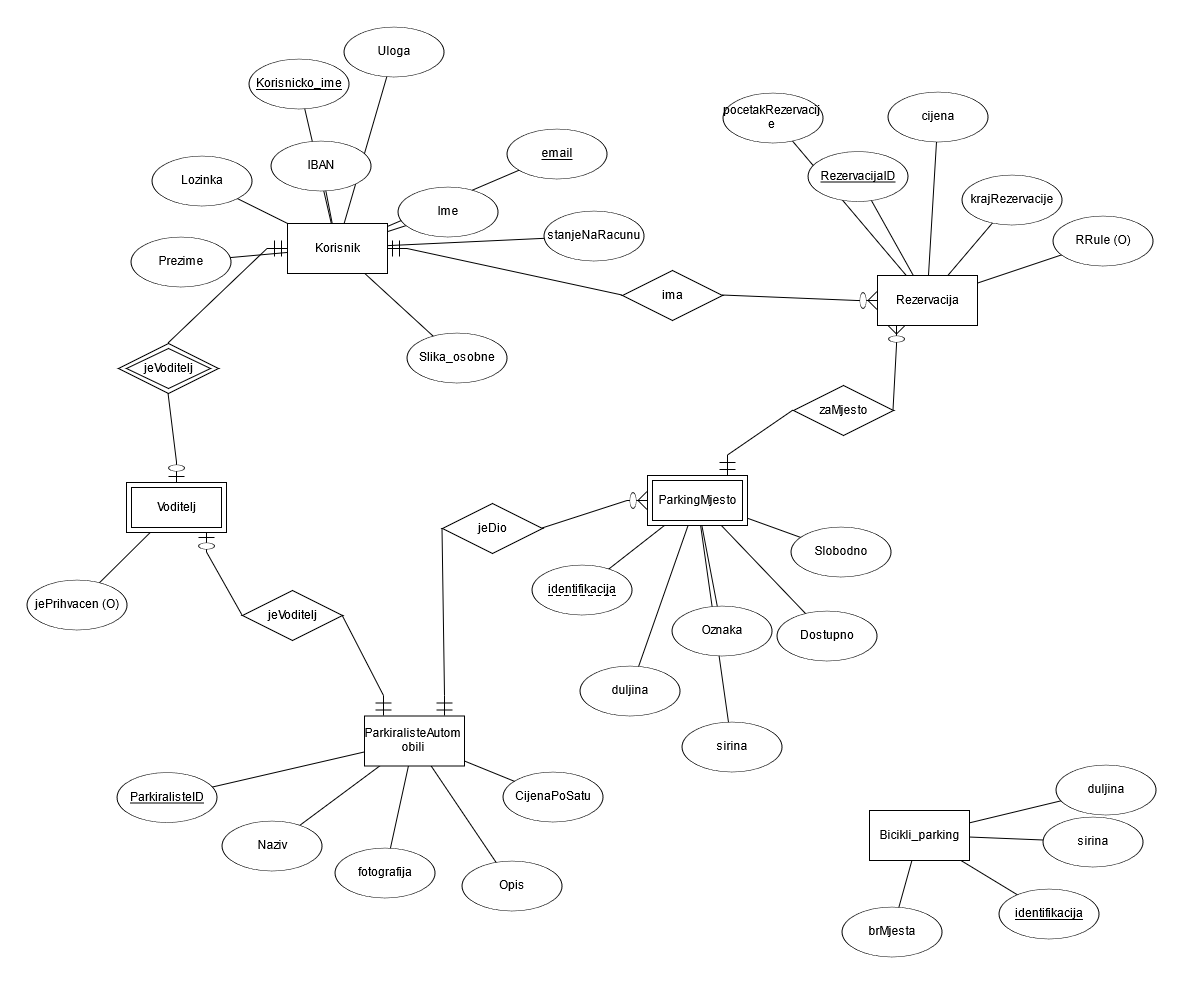
\includegraphics[width=\textwidth]{slike/erl.PNG} %veličina slike u odnosu na originalnu datoteku i pozicija slike
					\centering
					\caption{E-R dijagram baze podataka}
					\label{fig:erldijagram}
				\end{figure}
				
				\begin{figure}[H]
					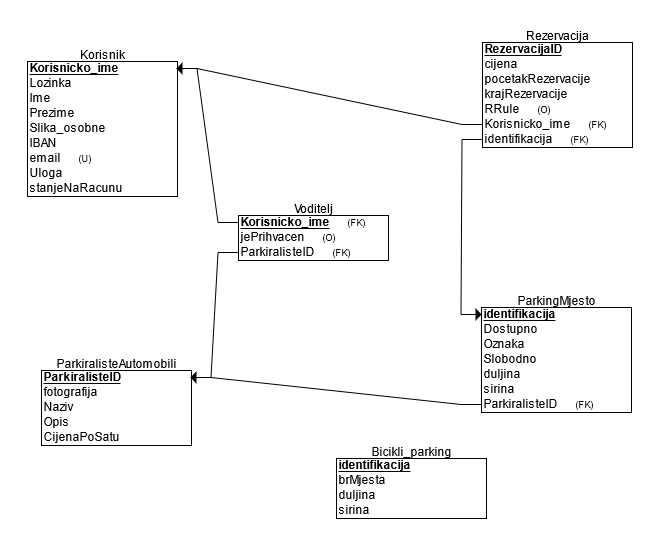
\includegraphics[scale=0.7]{slike/rlc.PNG} %veličina u odnosu na širinu linije
					\caption{Relacijska shema}
					\label{fig:relshema} %label mora biti drugaciji za svaku sliku
				\end{figure}
				
				
				
				
				
			
			
			
			
			
			\eject
			
			
		\section{Dijagram razreda}
		
			\textit{Potrebno je priložiti dijagram razreda s pripadajućim opisom. Zbog preglednosti je moguće dijagram razlomiti na više njih, ali moraju biti grupirani prema sličnim razinama apstrakcije i srodnim funkcionalnostima.}\\
			
			\textbf{\textit{dio 1. revizije}}\\
			
			\textit{Prilikom prve predaje projekta, potrebno je priložiti potpuno razrađen dijagram razreda vezan uz \textbf{generičku funkcionalnost} sustava. Ostale funkcionalnosti trebaju biti idejno razrađene u dijagramu sa sljedećim komponentama: nazivi razreda, nazivi metoda i vrste pristupa metodama (npr. javni, zaštićeni), nazivi atributa razreda, veze i odnosi između razreda.}\\
			
			\textbf{\textit{dio 2. revizije}}\\			
			
			\textit{Prilikom druge predaje projekta dijagram razreda i opisi moraju odgovarati stvarnom stanju implementacije}
			
			
			
			\eject
		
		\section{Dijagram stanja}
			
			
			\textbf{\textit{dio 2. revizije}}\\
			
			\textit{Potrebno je priložiti dijagram stanja i opisati ga. Dovoljan je jedan dijagram stanja koji prikazuje \textbf{značajan dio funkcionalnosti} sustava. Na primjer, stanja korisničkog sučelja i tijek korištenja neke ključne funkcionalnosti jesu značajan dio sustava, a registracija i prijava nisu. }
			
			
			\eject 
		
		\section{Dijagram aktivnosti}
			
			\textbf{\textit{dio 2. revizije}}\\
			
			 \textit{Potrebno je priložiti dijagram aktivnosti s pripadajućim opisom. Dijagram aktivnosti treba prikazivati značajan dio sustava.}
			
			\eject
		\section{Dijagram komponenti}
		
			\textbf{\textit{dio 2. revizije}}\\
		
			 \textit{Potrebno je priložiti dijagram komponenti s pripadajućim opisom. Dijagram komponenti treba prikazivati strukturu cijele aplikacije.}
	\chapter{Implementacija i korisničko sučelje}


\section{Korištene tehnologije i alati}


\hspace{0.67cm}Komunikacija u timu odvijala se putem aplikacija \underline{WhatsApp}\footnote{\url{https://www.whatsapp.com/}} i \underline{Discord}\footnote{\url{https://discord.com/}}.
Kao sustav za upravljanje izvornim kodom korišten je \underline{Git}\footnote{\url{https://git-scm.com/}}, distribuirani sustav kontrole verzija koji prati promjene u bilo kojem skupu datoteka. Udaljeni repozitorij projekta je dostupan na web platformi \underline{GitLab}\footnote{\url{https://about.gitlab.com/}}.

UML dijagrami su napravljeni u \underline{Visual Paradigm Online}\footnote{\url{https://www.visual-paradigm.com/}}, besplatnom alatu za crtanje.

Pri oblikovanju aplikacije za \textit{backend}  je korišten radni okvir \underline{Spring Boot}\footnote{\url{https://spring.io/projects/spring-boot/}} i jezik \underline{Java}\footnote{\url{https://www.java.com/en/}}. Spring Boot je otvoreni Java radni okvir namijenjen pojednostavljenoj izgradnji samostalnih, produkcijski orijentiranih Spring aplikacija. Pruža optimiziranu platformu za razvoj Java aplikacija s naglaskom na konvenciju umjesto konfiguracije, omogućavajući programerima brzo postavljanje i razvoj robusnih, skalabilnih i efikasnih aplikacija. Spring Boot dolazi s ugrađenim značajkama poput automatske konfiguracije, podrške za ugrađeni web poslužitelj i postavkama spremnim za produkcijsko okruženje. Java je objektno orijentirani i platformski neovisan programski jezik. Kod napisan u Javi može izvoditi na bilo kojem uređaju ili platformi s Java Virtual Machine (JVM). Java je poznata po svojoj prenosivosti, snažnoj podršci zajednice i obilnim bibliotekama, što je čini popularnim izborom za izgradnju različitih vrsta aplikacija.




Za implementaciju \textit{frontenda} koristili smo razvojno okruženje \underline{React}\footnote{\url{https://react.dev/}} i jezik \underline{JavaScript}\footnote{\url{https://www.javascript.com/}}. React je otvorena JavaScript biblioteka za izgradnju korisničkih sučelja. Omogućuje stvaranje ponovno upotrebljivih komponenti korisničkog sučelja, upravljanje njihovim vlastitim stanjem i učinkovito ažuriranje korisničkog sučelja putem virtualnog DOM-a. React slijedi jednosmjerni tok podataka, koristi JSX za sintaksu komponenata i široko se koristi zbog modularnosti i optimizacija performansi.
JavaScript je svestrani i objektno orijentirani jezik, uglavnom korišten za stvaranje dinamičnog i interaktivnog sadržaja na web stranicama. Podržava asinkrono programiranje i radi na različitim platformama, što ga čini ključnom tehnologijom u web razvoju. Osim u preglednicima, proširuje se i na druge domene, uključujući i izradu mobilnih aplikacija. 

\underline{LaTeX}\footnote{\url{https://www.latex-project.org/}} je sustav za stvaranje visokokvalitetnih dokumenata, posebno u znanstvenim i akademskim kontekstima. Koristi označavanje teksta pomoću naredbi kako bi se definirala struktura dokumenta i formatiranje. Korisnici pišu dokumente u običnom tekstu s ekstenzijom .tex i koriste LaTeX compiler za generiranje formatiranih izlaza, često u PDF formatu.


\eject 


\section{Ispitivanje programskog rješenja}




\subsection{Ispitivanje komponenti}

Ispitivanje komponenti provjerava ispravnost djelovanja pojedinih dijelova programa koji su mogući za odvojeno ispitivanje, poput pojedinačnih funkcija ili metoda unutar objekta. U ovom projektu koristimo JUnit i Mockito za implementaciju i izvođenje automatskih testova. JUnit je okvir za testiranje koji omogućuje definiranje, organiziranje i izvođenje testova kako bismo provjerili ispravnost funkcionalnosti naše aplikacije. Mockito je biblioteka koja nam omogućuje stvaranje lažnih objekata kako bismo simulirati njihovu funkcionalnost, omogućujući izolaciju jedinica koda i neovisno testiranje. Pomoću Mockito-a smo stvorili mock objekte za servise i repozitorije, što nam omogućuje precizno kontroliranje ponašanja tih objekata tijekom testiranja.

\begin{figure}[H]
	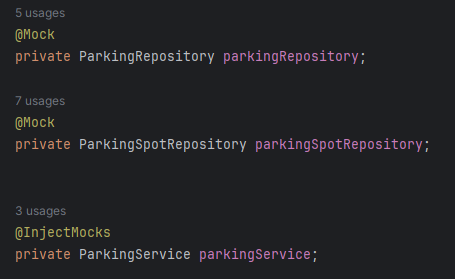
\includegraphics[width=\textwidth]{slike/mock.png} %veličina slike u odnosu na originalnu datoteku i pozicija slike
	\centering
	\caption{Stvaranje mock objekata}
	\label{fig:dijagramstanja}
\end{figure}



Ispitivanje komponenti za CreateKorisnikTest fokusira se na verifikaciju funkcionalnosti klase KorisnikService prilikom stvaranja novog korisnika. Testiraju se različiti scenariji, uključujući prepoznavanje već postojećeg emaila ili korisničkog imena te obrada null vrijednosti slike.

\begin{figure}[H]
	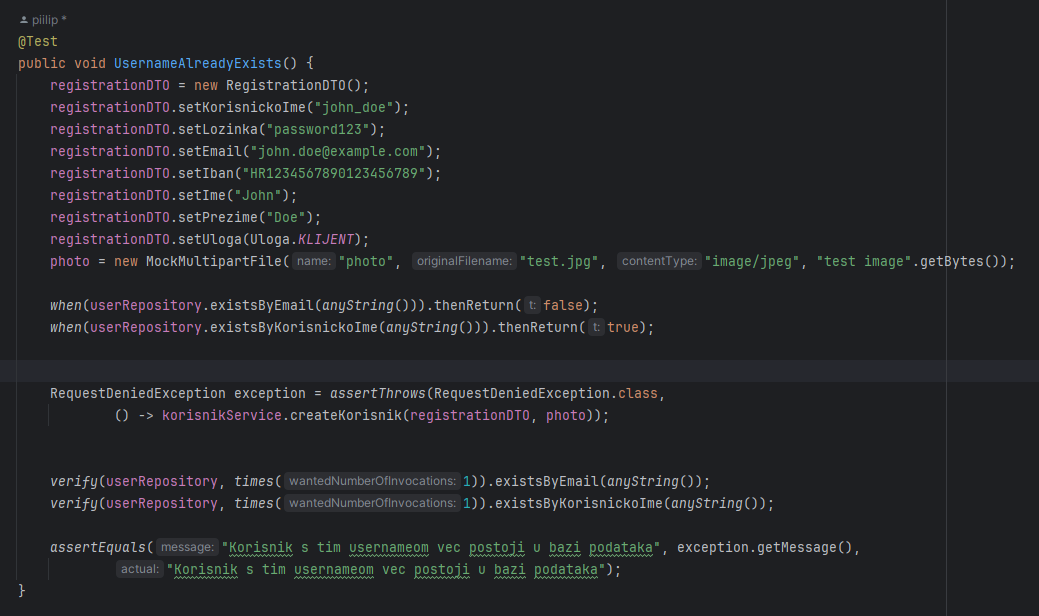
\includegraphics[width=\textwidth]{slike/username.png} %veličina slike u odnosu na originalnu datoteku i pozicija slike
	\centering
	\caption{1. ispitni slučaj za CreateKorisnikTest}
	\label{fig:dijagramstanja}
\end{figure}

\begin{figure}[H]
	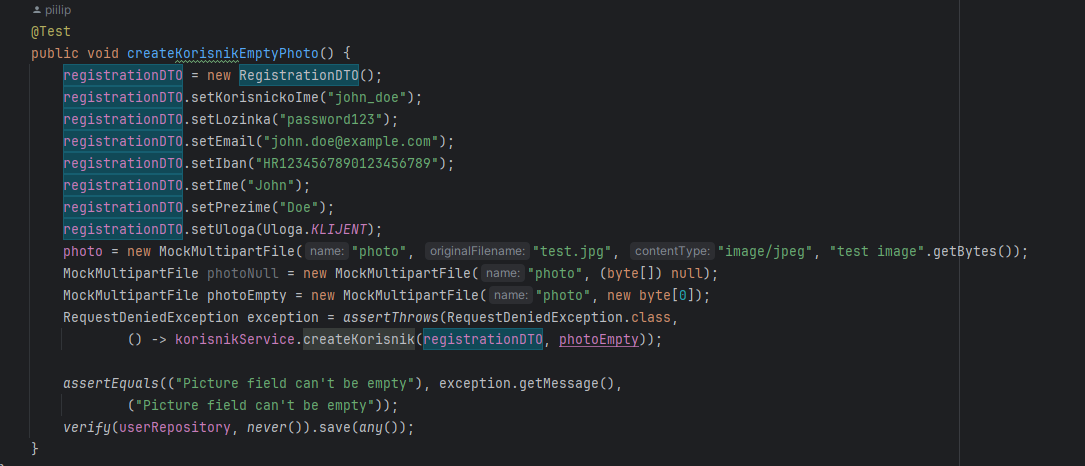
\includegraphics[width=\textwidth]{slike/korisnikslika.png} %veličina slike u odnosu na originalnu datoteku i pozicija slike
	\centering
	\caption{2. ispitni slučaj za CreateKorisnikTest}
	\label{fig:dijagramstanja}
\end{figure}

\begin{figure}[H]
	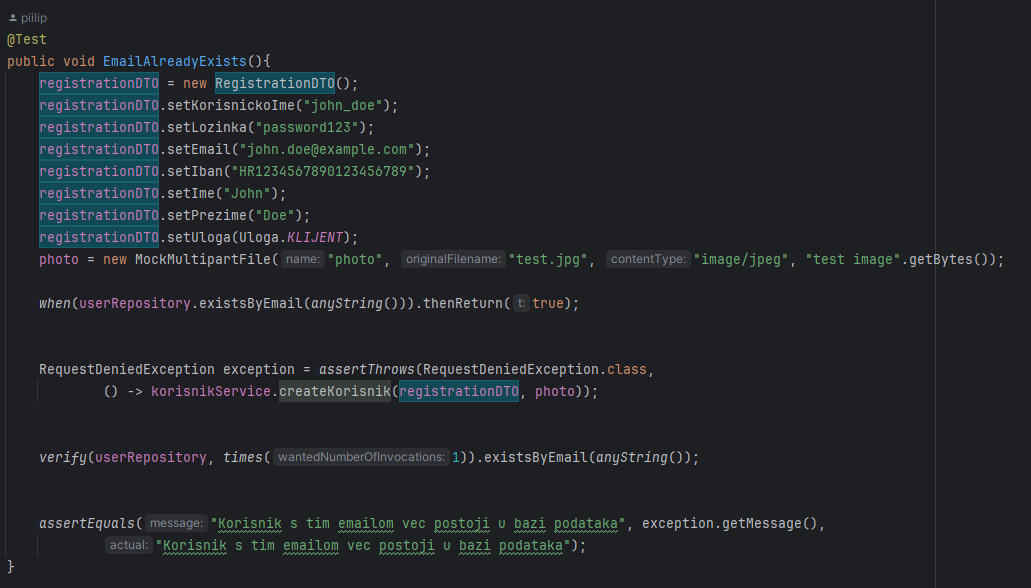
\includegraphics[width=\textwidth]{slike/email.png} %veličina slike u odnosu na originalnu datoteku i pozicija slike
	\centering
	\caption{3. ispitni slučaj za CreateKorisnikTest}
	\label{fig:dijagramstanja}
\end{figure}

Ispitivanje komponenti za UpdateKorisnikTest usmjereno je na verifikaciju funkcionalnosti metode updateKorisnik unutar klase KorisnikService. Testiraju se scenariji ažuriranja korisničkih podataka, uključujući promjenu korisničkog imena, imena, lozinke i slike.

\begin{figure}[H]
	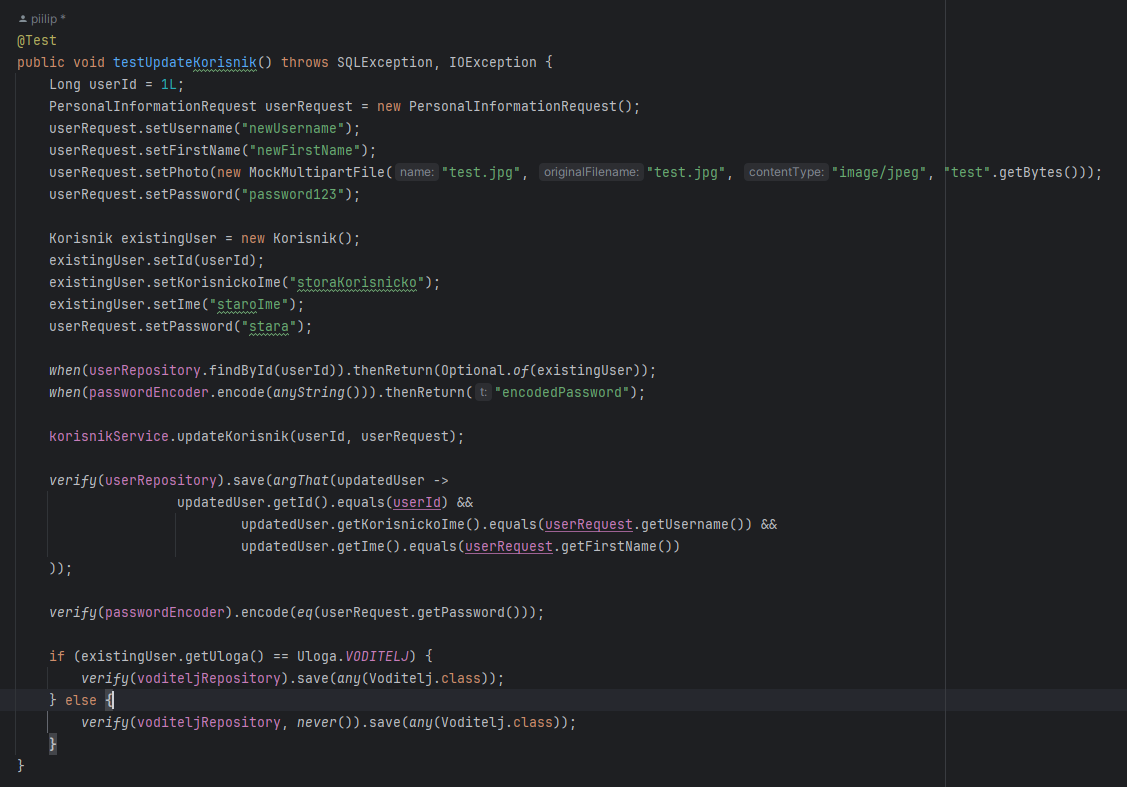
\includegraphics[width=\textwidth]{slike/testupdatekorisnik.png} %veličina slike u odnosu na originalnu datoteku i pozicija slike
	\centering
	\caption{1. ispitni slučaj za UpdateKorisnikTest}
	\label{fig:dijagramstanja}
\end{figure}


Ispitivanje komponenti za ParkingServiceTest usmjereno je na verifikaciju funkcionalnosti klase ParkingService. Fokusirano je na ispravno označavanje parkirnih mjesta kao rezervirana i ponašanje sustava u različitim scenarijima(verifikacija ispravnosti označavanja parkirnih mjesta kao rezervirana, provjera ponašanja sustava u slučaju nepostojećeg parkirališta, verifikacija ponašanja sustava kada je parkirno mjesto već označeno i testiranje ispravnosti dobivanja indeksa najmanje udaljenosti). Provjeravamo metodu markSpots koja je dio ParkingServicea. 
Ta metoda će pridružiti dana parkirališna mjesta s parkiralištem, osim u slučaju kad parkirno već pripada nekom drugom parkiralištu. U slučaju kad su sva mjesta uspješno rezervirana ta metoda vraća null vrijednost, a u suprotnom vraća listu onih mjesta koja nismo uspjeli rezervirati.
U testu markSpotsSuccess metode želimo provjeriti hoće li metoda vratiti null vrijednost, ako smo rezervirali sva mjesta. Testiramo samo s jednim parkingSpotom koje nema označen Parking, odnosno parkingSpot.getParking() == null i zbog toga očekujemo da će povratna vrijednost poziva markSpots biti null. 

\begin{figure}[H]
	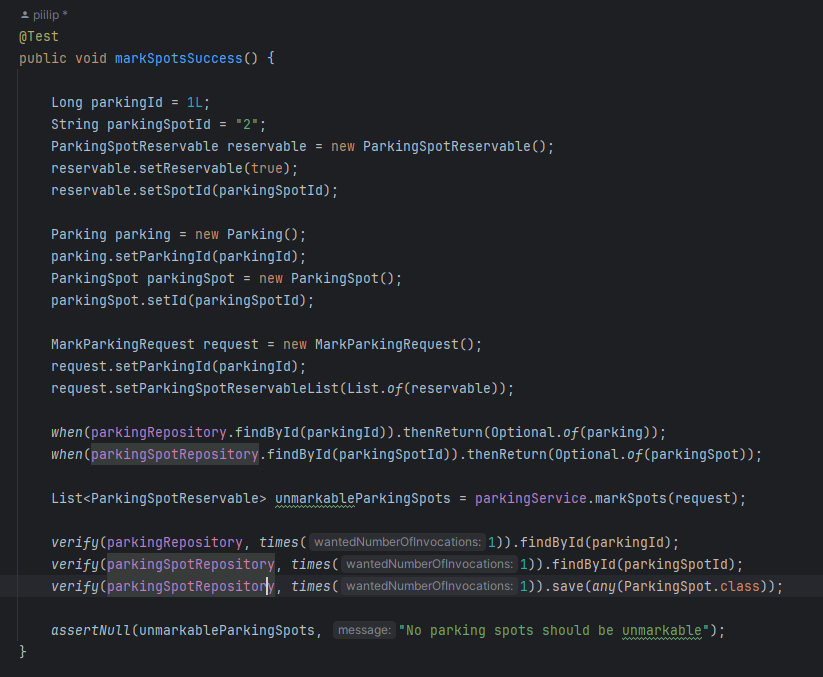
\includegraphics[width=\textwidth]{slike/markspotsuccess.png} %veličina slike u odnosu na originalnu datoteku i pozicija slike
	\centering
	\caption{1. ispitni slučaj za ParkingServiceTest}
	\label{fig:dijagramstanja}
\end{figure}


S testom markSpotsSomeFoundSomeNot testiramo slučaj kad imamo jedno ispravno i jedno neispravno mjesto. Odnosno kad imamo jedno mjesto koje već pripada nekom parkiralištu i jedno koje ne pripada. U tom slučaju bi trebali spremiti ispravno parkiralište (broj poziva parkingSpotRepository.save() bi trebao biti jedan) i vratiti neispravna mjesta.


\begin{figure}[H]
	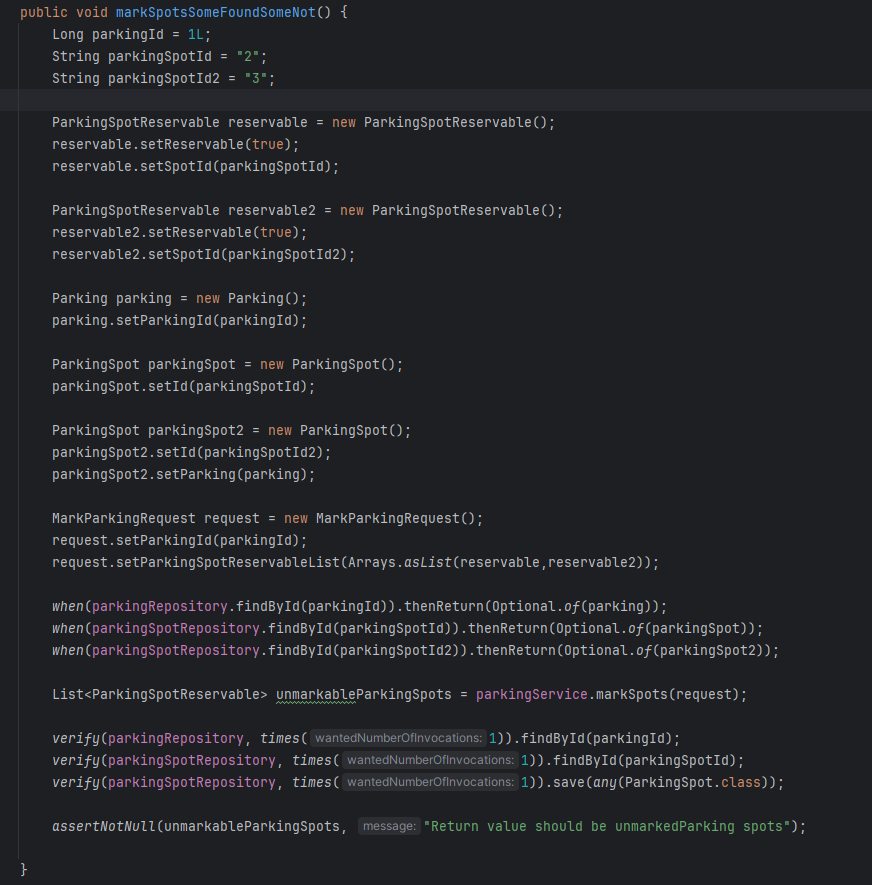
\includegraphics[width=\textwidth]{slike/markspotfound.png} %veličina slike u odnosu na originalnu datoteku i pozicija slike
	\centering
	\caption{2. ispitni slučaj za ParkingServiceTest}
	\label{fig:dijagramstanja}
\end{figure}

\begin{figure}[H]
	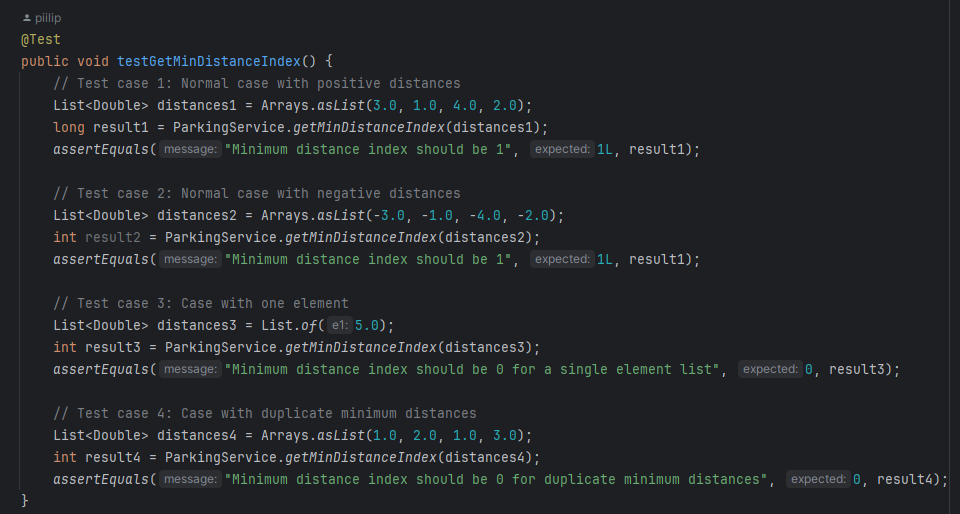
\includegraphics[width=\textwidth]{slike/testmindistance.png} %veličina slike u odnosu na originalnu datoteku i pozicija slike
	\centering
	\caption{3. ispitni slučaj za ParkingServiceTest}
	\label{fig:dijagramstanja}
\end{figure}

\begin{figure}[H]
	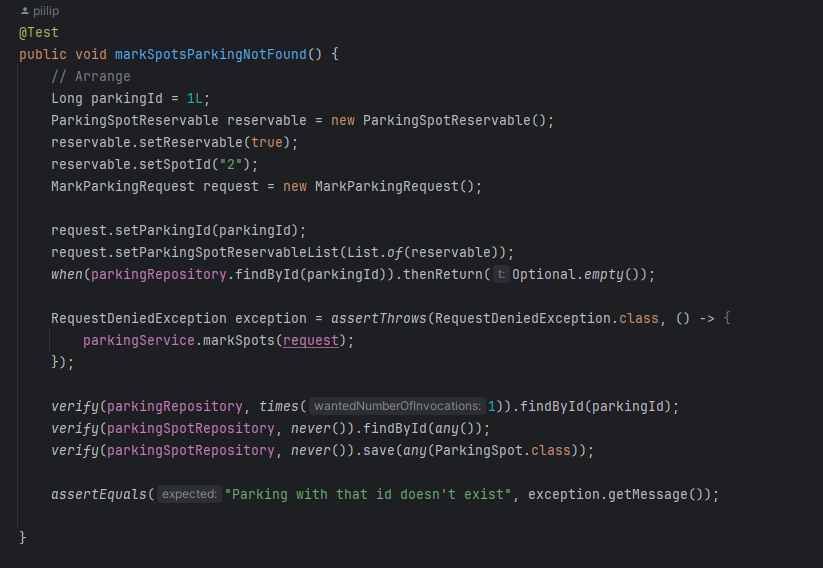
\includegraphics[width=\textwidth]{slike/markspotparking.png} %veličina slike u odnosu na originalnu datoteku i pozicija slike
	\centering
	\caption{4. ispitni slučaj za ParkingServiceTest}
	\label{fig:dijagramstanja}
\end{figure}


\begin{figure}[H]
	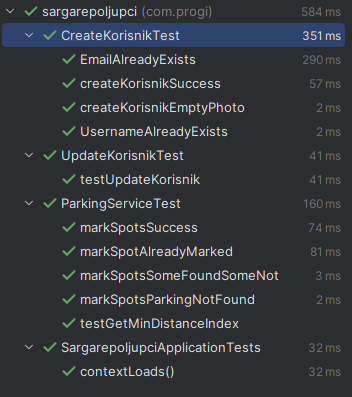
\includegraphics[width=\textwidth]{slike/results.png} %veličina slike u odnosu na originalnu datoteku i pozicija slike
	\centering
	\caption{Rezultati svih ispitnih slučajeva}
	\label{fig:dijagramstanja}
\end{figure}

\subsection{Ispitivanje sustava}

\eject 


\section{Dijagram razmještaja}


UML-dijagrami razmještaja (engl. deployment diagrams) su takoder vrsta strukturnih UML-dijagrama koji prikazuju fizičku arhitekturu i konfiguraciju razmještaja programskog sustava. Oni ilustriraju raspodjelu programskih komponenti, izvršnih datoteka i knjižnica na sklopovske čvorove ili virtualna izvršna okruženja.
Na poslužiteljskom računalu nalaze se Web poslužitelj i poslužitelj baze podataka. Korisnik do web aplikacije dolazi preko web preglednika pri čemu mobilna aplikacija komunicira s poslužiteljem pomoću protokola HTTP. Osim s korisnikom, web poslužitelj komunicira i s OSRM pomoću protokola HTTP.

\vspace{5cm}

\begin{figure}[H]
	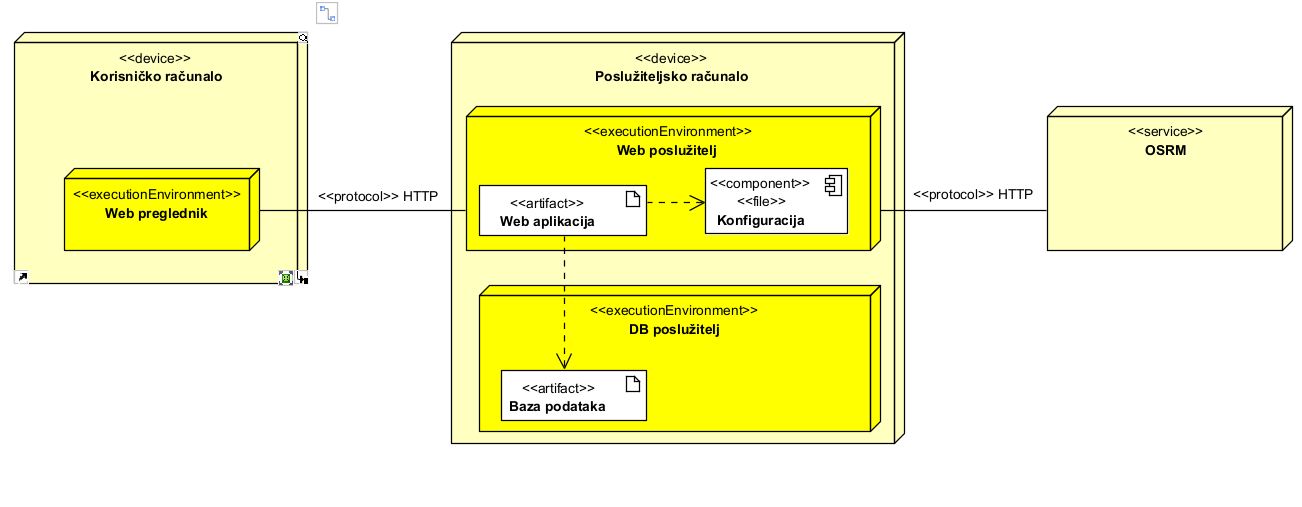
\includegraphics[width=\textwidth]{slike/dijagram_razmjestaja.png} %veličina slike u odnosu na originalnu datoteku i pozicija slike
	\centering
	\caption{Dijagram razmještaja}
	\label{fig:dijagramaktivnosti}
\end{figure}
\eject 

\section{Upute za puštanje u pogon}

Prvo, preuzmite glavnu granu repozitorija ove web aplikacije putem naredbe "git pull" s GitLab-a.

Za implementaciju na Renderu, preporučljivo je stvoriti račun na GitHub-u ili GitLab-u i povezati ga s Renderom. Nakon stvaranja računa, možete dodati web aplikaciju kao novi projekt na svom računu.

Što se tiče baze podataka na Renderu, prijavite se, kliknite na gumb "New" u gornjem desnom kutu i odaberite opciju "PostgreSQL". Unesite identifikacijske podatke i konfiguracijske informacije, poput lako prepoznatljivog imena baze (koje će se prikazivati u Renderu), stvarnog imena baze podataka, korisničkog imena i odabira regije. Ostavite verziju PostgreSQL-a na zadanim postavkama, osim ako imate posebne zahtjeve. Odaberite plan ovisno o očekivanom prometu na stranici i pritisnite "Create Database". Potrebni podaci za povezivanje s bazom bit će dostupni na vašem "dashboardu" pod "Connections".

Opcionalno punjenje baze podataka podacima može se izvršiti pomoću već pripremljenih informacija koje odgovaraju strukturi navedenoj u odjeljku "Baza podataka". Korisno je koristiti PGAdmin ili sličan alat za ovu svrhu. Slijede upute o tome kako to postići korištenjem navedenog alata. Nakon što otvorite PGAdmin, desnim klikom odaberite ikonu "Servers" s lijeve strane. Zatim odaberite opciju "Create" i popunite obrazac na sljedeći način: unesite ime baze koje ste odabrali u polje "Name" pri kreaciji baze, dok pod "Database" upišete isto ime koje ste koristili prilikom stvaranja baze.

U polju "Host-name/address", unesite informacije o bazi u formatu "Hostname.Region-postgres.render.com", pri čemu "Region" prepisujete malim slovima (samo prvu riječ). Pod "Port" upišite broj iz "Connections" pod "Port", dok za "Username" koristite isti podatak koji ste koristili pri stvaranju baze. Kliknite "Save" za pohranu. Prilikom svake buduće konekcije, sustav će tražiti nasumično generiranu "Password" koju ste dobili od Rendera. Ako želite, možete postaviti automatsku vezu između vašeg PGAdmina i baze.

Što se tiče ubacivanja podataka, navigirajte do spojenog servera, otvorite listu baza podataka i desnim klikom odaberite ciljanu bazu. Odaberite opciju "Restore" i ispunite obrazac kako biste učitali svoju sigurnosnu kopiju (backup) u željenom formatu.

Deployanje backend aplikacije na Render:

Za početak, kliknite na opciju "New" i odaberite "Web Service". Ako ste prijavljeni s GitHub ili GitLab računom, imat ćete priliku odabrati projekt koji želite deployati. Kliknite na "Connect" pored odabranog projekta. Unesite jedinstveno ime pod nazivom "PodName" za vaš web servis, koje će istovremeno poslužiti i kao dio URL-a za pristup stranici (u suprotnom, Render će automatski dodati brojeve kako bi ga učinio jedinstvenim). Odaberite "Region" gdje želite da bude server vaše web aplikacije te specificirajte "Branch" koji želite deployati.

U polje "Dockerfile Path", unesite ./docker/maven/Dockerfile. U naprednim postavkama dodajte potrebne okolišne varijable, na primjer, za bazu podataka ili privatne podatke kao što su adrese e-pošte koje ćete koristiti za slanje registracijskih e-mailova novim korisnicima.

Također, možete čvrsto definirati ove varijable u datoteci application.properties u resursima na backendu. Obratite pažnju da Render ponekad zahtijeva više pokušaja deployanja dok ne uskladi varijable.

Osigurajte da imate potrebne podatke o bazi (isti podaci koje ste koristili za povezivanje putem PGAdmina, uključujući korisničko ime i lozinku za aplikaciju).

Postupak deployanja frontenda na Render platformi zahtijeva nekoliko koraka. Počnite klikom na gumb "New" i odaberite opciju "Web Service". Ako ste povezani s GitHub ili GitLab računom, odaberite projekt koji želite deployati i pritisnite "Connect". Unesite jedinstveno ime za vaš web servis, koje će također biti dio URL-a pristupa stranici. Odaberite željenu regiju za server i granu koju želite deployati.

 U odjeljku "Environment" odaberite "Node", a za "Build command" koristite "yarn build". Možete prilagoditi naredbe u "package.json" datoteci frontenda pod "scripts". "Start command" trebao bi biti "yarn start-prod".

Proširite "advanced" opcije i dodajte environment varijable prema potrebi. Ponekad može biti potrebno više puta deployati frontend dok Render ne izgradi sve. Ako želite olakšati postupak, možete promijeniti "target" atribut u datoteci "setupProxy.js" na URL vašeg deployanog backenda. Isto tako, prilagodite isto u datoteci "app.js" u frontend direktoriju. Nazivi datoteka su jedinstveni, pa ih možete pronaći u Exploreru datoteka.

\eject 
	\chapter{Zaključak i budući rad}
		
		\textbf{\textit{dio 2. revizije}}\\
		
		 \textit{U ovom poglavlju potrebno je napisati osvrt na vrijeme izrade projektnog zadatka, koji su tehnički izazovi prepoznati, jesu li riješeni ili kako bi mogli biti riješeni, koja su znanja stečena pri izradi projekta, koja bi znanja bila posebno potrebna za brže i kvalitetnije ostvarenje projekta i koje bi bile perspektive za nastavak rada u projektnoj grupi.}
		
		 \textit{Potrebno je točno popisati funkcionalnosti koje nisu implementirane u ostvarenoj aplikaciji.}
		
		\eject 
	\chapter*{Popis literature}
		\addcontentsline{toc}{chapter}{Popis literature}
	 	
 		\textbf{\textit{Kontinuirano osvježavanje}}
	
		\textit{Popisati sve reference i literaturu koja je pomogla pri ostvarivanju projekta.}
		
		
		\begin{enumerate}
			
			
			\item  Programsko inženjerstvo, FER ZEMRIS, \url{http://www.fer.hr/predmet/proinz}
			
			\item  I. Sommerville, "Software engineering", 8th ed, Addison Wesley, 2007.
			
			\item  T.C.Lethbridge, R.Langaniere, "Object-Oriented Software Engineering", 2nd ed. McGraw-Hill, 2005.
			
			\item  I. Marsic, Software engineering book``, Department of Electrical and Computer Engineering, Rutgers University, \url{http://www.ece.rutgers.edu/~marsic/books/SE}
			
			\item  The Unified Modeling Language, \url{https://www.uml-diagrams.org/}
			
			\item  Astah Community, \url{http://astah.net/editions/uml-new}
		\end{enumerate}
		
		 
	
	
	\begingroup
	\renewcommand*\listfigurename{Indeks slika i dijagrama}
	%\renewcommand*\listtablename{Indeks tablica}
	%\let\clearpage\relax
	\listoffigures
	%\vspace{10mm}
	%\listoftables
	\endgroup
	\addcontentsline{toc}{chapter}{Indeks slika i dijagrama}


	
	\eject 
		
	\chapter*{Dodatak: Prikaz aktivnosti grupe}
		\addcontentsline{toc}{chapter}{Dodatak: Prikaz aktivnosti grupe}
		
		\section*{Dnevnik sastajanja}
		
		\textbf{\textit{Kontinuirano osvježavanje}}\\
		
		 \textit{U ovom dijelu potrebno je redovito osvježavati dnevnik sastajanja prema predlošku.}
		
		\begin{packed_enum}
			\item  sastanak
			
			\item[] \begin{packed_item}
				\item Datum: u ovom formatu: \today
				\item Prisustvovali: I.Prezime, I.Prezime
				\item Teme sastanka:
				\begin{packed_item}
					\item  opis prve teme
					\item  opis druge teme
				\end{packed_item}
			\end{packed_item}
			
			\item  sastanak
			\item[] \begin{packed_item}
				\item Datum: u ovom formatu: \today
				\item Prisustvovali: I.Prezime, I.Prezime
				\item Teme sastanka:
				\begin{packed_item}
					\item  opis prve teme
					\item  opis druge teme
				\end{packed_item}
			\end{packed_item}
			
			%
			
		\end{packed_enum}
		
		\eject
		\section*{Tablica aktivnosti}
		
			\textbf{\textit{Kontinuirano osvježavanje}}\\
			
			 \textit{Napomena: Doprinose u aktivnostima treba navesti u satima po članovima grupe po aktivnosti.}

			\begin{longtblr}[
					label=none,
				]{
					vlines,hlines,
					width = \textwidth,
					colspec={X[7, l]X[1, c]X[1, c]X[1, c]X[1, c]X[1, c]X[1, c]X[1, c]}, 
					vline{1} = {1}{text=\clap{}},
					hline{1} = {1}{text=\clap{}},
					rowhead = 1,
				} 
			
				\SetCell[c=1]{c}{} & \SetCell[c=1]{c}{\rotatebox{90}{\textbf{Ime Prezime voditelja}}} & \SetCell[c=1]{c}{\rotatebox{90}{\textbf{Ime Prezime }}} &	\SetCell[c=1]{c}{\rotatebox{90}{\textbf{Ime Prezime }}} & \SetCell[c=1]{c}{\rotatebox{90}{\textbf{Ime Prezime }}} &	\SetCell[c=1]{c}{\rotatebox{90}{\textbf{Ime Prezime }}} & \SetCell[c=1]{c}{\rotatebox{90}{\textbf{Ime Prezime }}} &	\SetCell[c=1]{c}{\rotatebox{90}{\textbf{Ime Prezime }}} \\  
				Upravljanje projektom 		&  &  &  &  &  &  & \\ 
				Opis projektnog zadatka 	&  &  &  &  &  &  & \\ 
				
				Funkcionalni zahtjevi       &  &  &  &  &  &  &  \\ 
				Opis pojedinih obrazaca 	&  &  &  &  &  &  &  \\ 
				Dijagram obrazaca 			&  &  &  &  &  &  &  \\ 
				Sekvencijski dijagrami 		&  &  &  &  &  &  &  \\ 
				Opis ostalih zahtjeva 		&  &  &  &  &  &  &  \\ 

				Arhitektura i dizajn sustava	 &  &  &  &  &  &  &  \\ 
				Baza podataka				&  &  &  &  &  &  &   \\ 
				Dijagram razreda 			&  &  &  &  &  &  &   \\ 
				Dijagram stanja				&  &  &  &  &  &  &  \\ 
				Dijagram aktivnosti 		&  &  &  &  &  &  &  \\ 
				Dijagram komponenti			&  &  &  &  &  &  &  \\ 
				Korištene tehnologije i alati 		&  &  &  &  &  &  &  \\ 
				Ispitivanje programskog rješenja 	&  &  &  &  &  &  &  \\ 
				Dijagram razmještaja			&  &  &  &  &  &  &  \\ 
				Upute za puštanje u pogon 		&  &  &  &  &  &  &  \\  
				Dnevnik sastajanja 			&  &  &  &  &  &  &  \\ 
				Zaključak i budući rad 		&  &  &  &  &  &  &  \\  
				Popis literature 			&  &  &  &  &  &  &  \\  
				&  &  &  &  &  &  &  \\ \hline 
				\textit{Dodatne stavke kako ste podijelili izradu aplikacije} 			&  &  &  &  &  &  &  \\ 
				\textit{npr. izrada početne stranice} 				&  &  &  &  &  &  &  \\  
				\textit{izrada baze podataka} 		 			&  &  &  &  &  &  & \\  
				\textit{spajanje s bazom podataka} 							&  &  &  &  &  &  &  \\ 
				\textit{back end} 							&  &  &  &  &  &  &  \\  
				 							&  &  &  &  &  &  &\\ 
			\end{longtblr}
					
					
		\eject
		\section*{Dijagrami pregleda promjena}
		
		\textbf{\textit{dio 2. revizije}}\\
		
		\textit{Prenijeti dijagram pregleda promjena nad datotekama projekta. Potrebno je na kraju projekta generirane grafove s gitlaba prenijeti u ovo poglavlje dokumentacije. Dijagrami za vlastiti projekt se mogu preuzeti s gitlab.com stranice, u izborniku Repository, pritiskom na stavku Contributors.}
		
	


\end{document} %naredbe i tekst nakon ove naredbe ne ulaze u izgrađen dokument 


